\documentclass[UTF8,a4paper,12pt,fontset=fandol]{ctexart}

\usepackage{amsmath}
\usepackage{amssymb}
\usepackage{bm}
\usepackage{graphicx}
\usepackage{booktabs}
\usepackage{tabularx}
\usepackage{array}
\usepackage[section]{placeins}
\usepackage[hidelinks]{hyperref}

\newcolumntype{Y}{>{\raggedright\arraybackslash}X}
\renewcommand{\arraystretch}{1.18}
\setlength{\emergencystretch}{2em}

\title{基于能谱支对齐可学习多相位 PINN 的含时 Dirac 方程求解研究\\
\large 研究介绍与阶段性报告}
\author{}
\date{2026年9月1日}

\begin{document}

\maketitle

\begin{quote}
\noindent\textbf{当前进度：}
理论分析、单波数验证、方法构造、机制消融、双波数推广和连续波包实验均已完成；下一阶段研究外势导致的动量耦合。
\end{quote}

\begin{abstract}
本研究考察物理信息神经网络求解含时 Dirac 方程时的长时间相位逼近问题。对于正、负能谱支的叠加态，单一共同相位表示难以同时分离符号相反的快速时间相位，因而在固定网络规模与训练预算下出现精度退化。为此，本文提出能谱支对齐的可学习双相位网络 LTPB。该方法首先依据自由 Dirac 哈密顿量的谱分解，将旋量波函数投影到正、负能本征子空间，随后分别表示两支的实振幅与相位函数。单波数、等参数消融和双波数实验表明，能谱支对齐与逐支相位表示具有互补作用。进一步构造的共享谱 LTPB 在固定参数规模下统一表示 33 个傅里叶模态，并在未参与训练的波数中点处保持正确的色散相位。与一般 Dirac-PINN 及单一共同相位 CPA 表示相比，该结构可能通过显式分离快速相位而改善混合能谱态的训练条件；相对于成熟的谱方法，其潜在价值主要体现在连续代理表示、稀疏观测融合和参数反演。后一类优势尚需通过外势、含噪数据及计算成本实验加以检验。
\end{abstract}

\section{研究问题}

考虑一维含时 Dirac 方程
\begin{equation}
i\hbar\partial_t\psi=
\left(-i\hbar c\sigma_x\partial_x+mc^2\sigma_z+V(x,t)I_2\right)\psi,
\qquad
\psi=(\psi_1,\psi_2)^{\mathsf T}.
\end{equation}
由 Dirac 哈密顿量的厄米性可导出概率密度、概率流密度及相应的连续性方程：
\begin{equation}
\rho=\psi^\dagger\psi,
\qquad
j=c\psi^\dagger\sigma_x\psi,
\qquad
\partial_t\rho+\partial_xj=0.
\end{equation}

令旋量波函数具有共同相位函数 $S$，
\begin{equation}
\psi=Ae^{iS/\hbar},
\end{equation}
代入上述定义可得
\begin{equation}
\rho=A^\dagger A,
\qquad
j=cA^\dagger\sigma_xA.
\end{equation}
可见，作为整体 $U(1)$ 相位的 $S$ 在 $\rho$ 与 $j$ 中约去。若将两个旋量分量分别写成
\begin{equation}
\psi_j=a_je^{iS_j/\hbar},
\end{equation}
则
\begin{equation}
j=2ca_1a_2\cos\!\left(\frac{S_2-S_1}{\hbar}\right),
\end{equation}
由此可见，概率流密度对旋量内部的相对相位 $(S_2-S_1)/\hbar$ 敏感。自由 Dirac 哈密顿量的正、负能本征态分别含有时间因子 $e^{-iEt}$ 与 $e^{+iEt}$。单一共同相位至多吸收其中一支的快速时间变化，另一支的高频振荡仍须由复振幅网络表征。

本文所称的性能退化，特指\textbf{固定网络规模与训练预算下的优化困难和逼近误差增长}。单一共同相位表示仍具有容纳目标解的函数表示能力。

\section{总体研究路线}

\begin{table}[htbp]
\centering
\small
\caption{总体研究路线与当前状态}
\begin{tabularx}{\textwidth}{@{}c l c Y@{}}
\toprule
阶段 & 内容 & 状态 & 研究结论 \\
\midrule
1 & 理论分析 & 已完成 & 共同相位函数不直接表征正、负能谱支之间的相对相位。 \\
2 & 单波数退化检验 & 已完成 & CPA-PINN 在单一正能谱支上精度较高，在混合能谱态上改善幅度显著减小。 \\
3 & LTPB 方法构造 & 已完成 & 逐支设置可学习相位可准确表示混合能谱态的时间演化。 \\
4 & 结构消融 & 已完成 & 能谱支对齐与逐支相位表示共同决定当前基准中的精度。 \\
5 & 双波数实验 & 已完成 & 相位表示已由两个频率分量推广至四个能谱分量。 \\
6 & 连续波包实验 & 已完成 & 共享谱网络可统一表示 33 个模态并插值至未训练波数。 \\
7 & 外势或散射 & 下一阶段 & 检验动量通道发生耦合后的适用性。 \\
8 & 稀疏含噪数据 & 待开展 & 考察状态重构和参数反演能力。 \\
9 & 完整基准评测 & 待开展 & 与现代 PINN 及传统数值方法比较精度、稳定性和计算成本。 \\
10 & 论文整理 & 待开展 & 形成理论机制、算法结构、消融验证、适用范围和数据应用的完整论证。 \\
\bottomrule
\end{tabularx}
\end{table}

\section{阶段一：理论分析}

\subsection{自由能谱支}

在自然单位制 $\hbar=c=1$ 下，波数为 $k$ 的自由 Dirac 哈密顿量在傅里叶表象中写成
\begin{equation}
H(k)=k\sigma_x+m\sigma_z,
\qquad
H(k)u_\pm=\pm E_k u_\pm,
\qquad
E_k=\sqrt{k^2+m^2}.
\end{equation}
其本征值为 $\pm E_k$，相应本征旋量记作 $u_\pm(k)$。正、负能谱支的叠加态可写为
\begin{equation}
\psi_\eta(x,t)=
\frac{e^{ikx}}{\sqrt{L(1+\eta^2)}}
\left(u_+e^{-iE_kt}+\eta u_-e^{+iE_kt}\right).
\end{equation}
当 $\eta=1$ 时，总范数保持不变，概率流密度中仍含有频率为 $2E_k$ 的干涉项。这一单模叠加态给出了检验支间相对相位逼近能力的最简模型。

\subsection{守恒约束的辨识能力}

记 Dirac 方程残差为 $R_D=i\partial_t\psi-H_D\psi$。直接计算可得
\begin{equation}
\partial_t\rho+\partial_xj
=2\operatorname{Im}(\psi^\dagger R_D).
\end{equation}
该恒等式表明，连续性方程给出方程残差在 $\psi$ 方向上的一个实投影；总范数与总能量则属于积分约束。上述守恒条件有助于限制整体演化，却不足以单独确定局域的支间相对相位。据此，后续参数化显式区分正、负能谱支的快速时间相位。

\section{阶段二：单一共同相位 CPA 表示的迁移检验}

\subsection{实验条件}

取 $m=5$、$k=2$、$T=5$、周期区间 $L=2\pi$，比较：
\begin{itemize}
  \item \texttt{Case P}：仅含正能谱支；
  \item \texttt{Case M}：正、负能谱支等权叠加。
\end{itemize}
各模型统一采用 4 个隐藏层、每层 64 个神经元的 \texttt{tanh} 网络；Adam 优化进行 5000 步，每步选取 1024 个配点。各可训练模型采用 3 个随机种子重复计算。

\subsection{结果}

\begin{table}[htbp]
\centering
\footnotesize
\caption{单一共同相位 CPA 表示的迁移检验结果}
\begin{tabular}{@{}lcccc@{}}
\toprule
模型 &
\shortstack{Case P\\波函数误差} &
\shortstack{Case M\\波函数误差} &
\shortstack{Case M\\流密度误差} &
\shortstack{Case M\\保真度} \\
\midrule
Vanilla & 0.9228 & 0.9452 & 0.9693 & 0.2254 \\
SP-CPA & \textbf{0.0067} & 0.7991 & 0.9392 & 0.5935 \\
SP-CPA-Conservative & 0.0111 & 1.0785 & 1.0698 & 0.1631 \\
解析双频参考模型 & 0.0079 & \textbf{0.0062} & \textbf{0.0105} & 0.999990 \\
\bottomrule
\end{tabular}
\end{table}

\begin{figure}[!htbp]
\centering
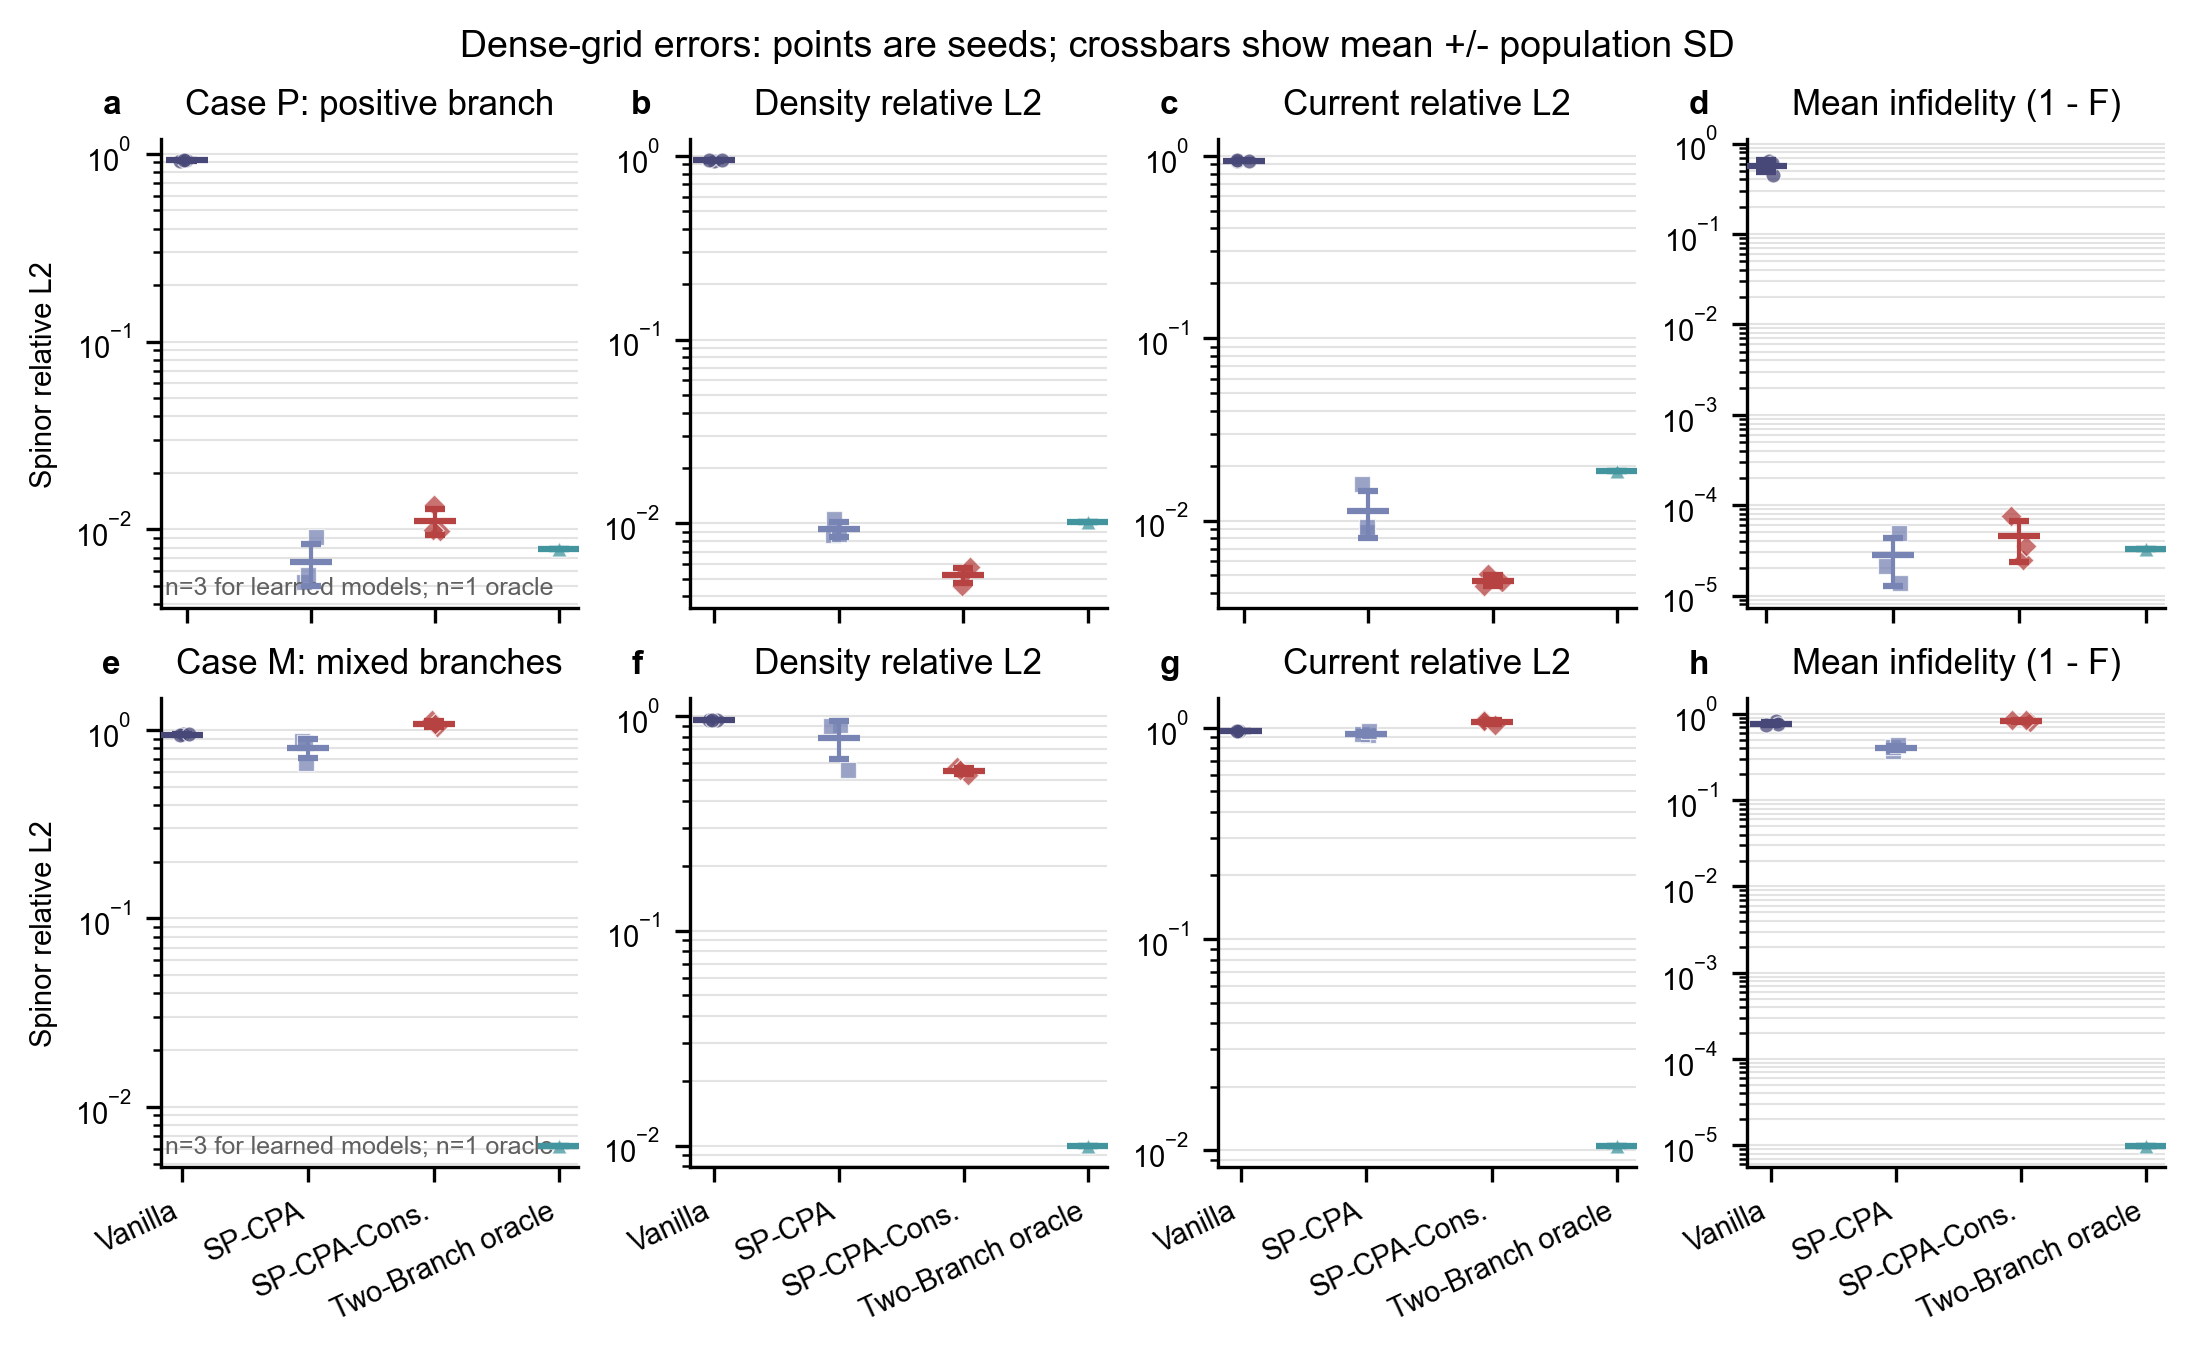
\includegraphics[width=0.88\textwidth]{results/figures/01_main_metric_comparison.png}
\caption{单一共同相位表示在纯正能谱支上获得较高精度，在正、负能谱支叠加态上的改善幅度显著减小。}
\label{fig:cpa-main}
\end{figure}

\begin{figure}[!htbp]
\centering
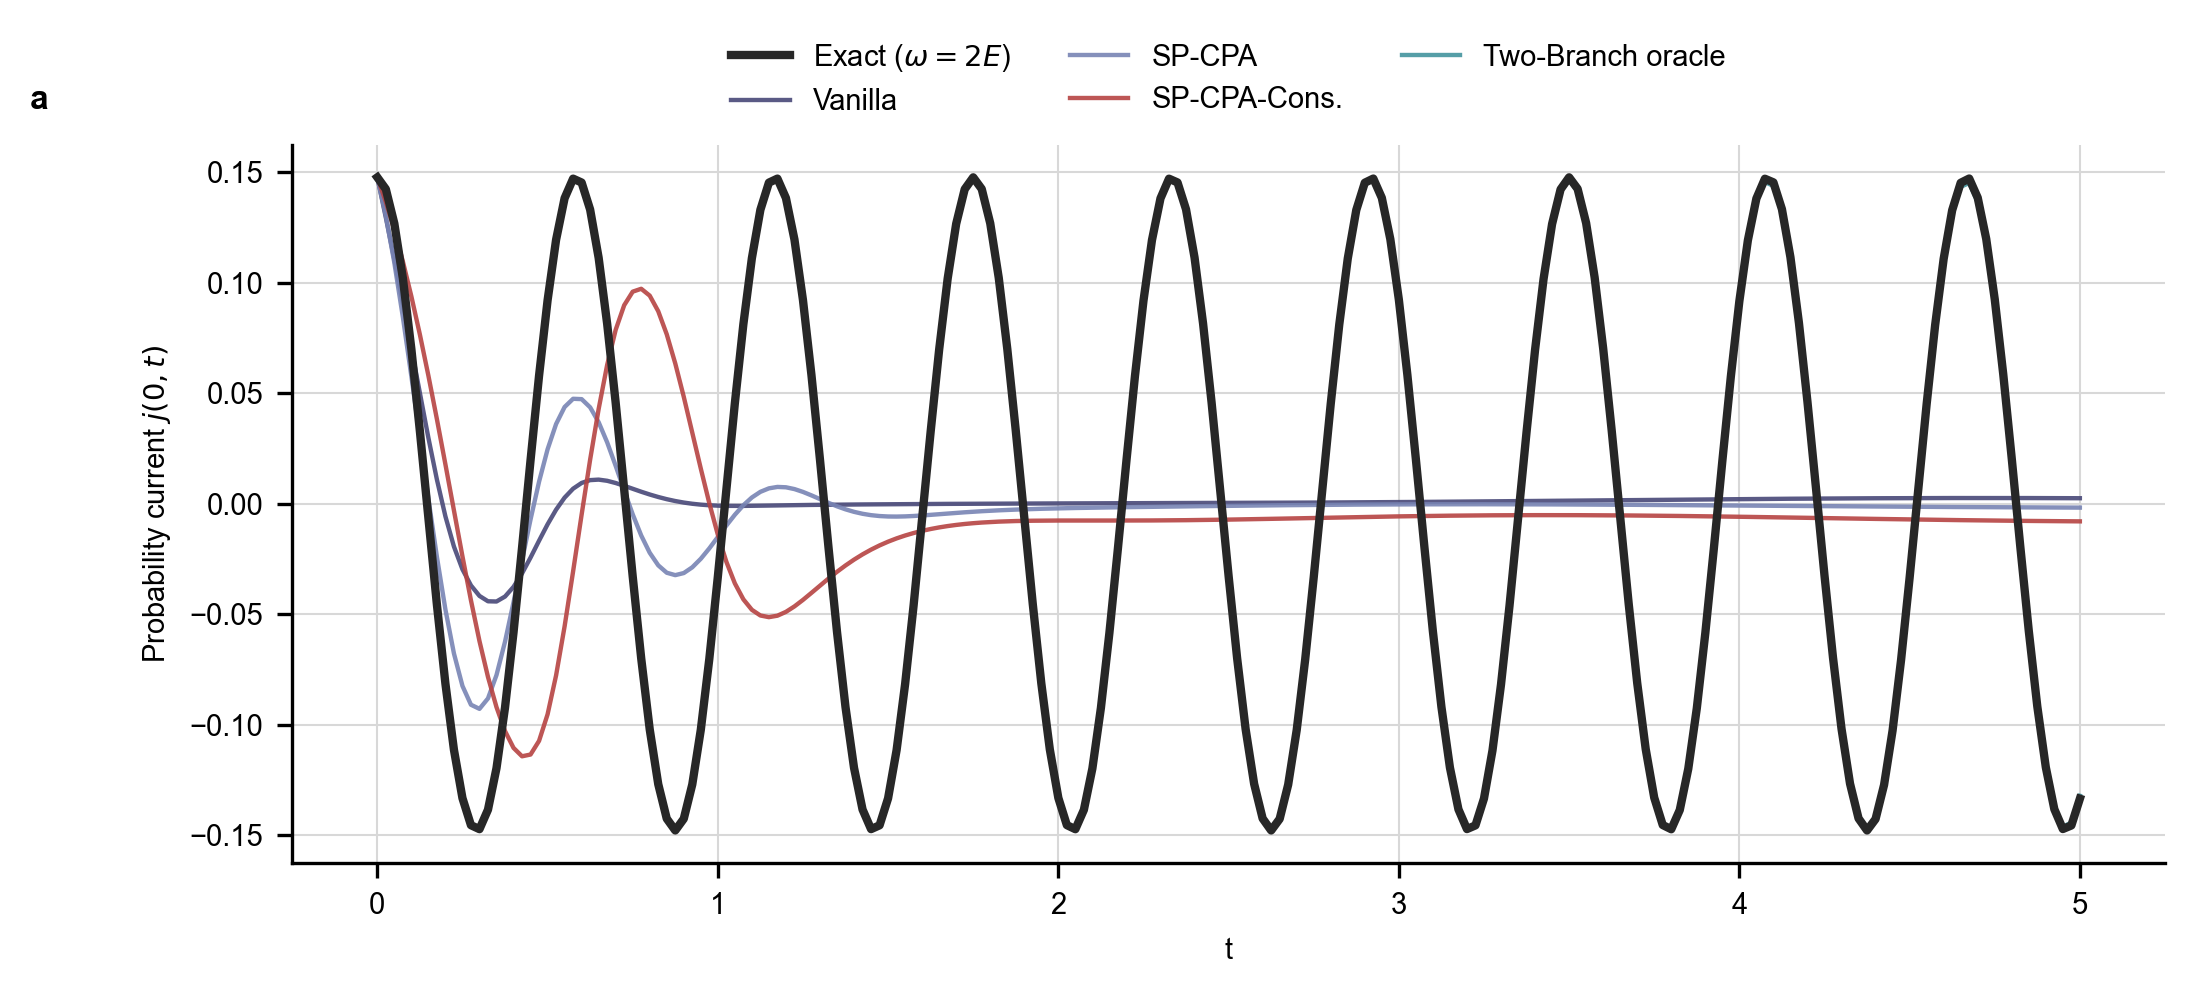
\includegraphics[width=0.88\textwidth]{results/figures/02_case_M_current_x0.png}
\caption{SP-CPA 对支间相干所产生的快速概率流振荡给出较大误差。}
\label{fig:cpa-current}
\end{figure}

相对于 Vanilla，SP-CPA 在 Case P 中将旋量波函数相对误差降低 $99.3\%$，在 Case M 中的降幅为 $15.5\%$。加入连续性、范数和能量损失后，概率流密度及支间相对相位的误差未见改善。错相解析构造进一步表明，即使整体守恒量接近精确值，局域波函数与概率流密度仍可能具有显著偏差。

\noindent\textbf{阶段结论：}
单一共同相位 CPA 表示在纯能谱支问题中具有良好效果；对于正、负能谱支叠加态，其快速相位分离作用受到限制，固定预算下的训练精度随之下降。

\section{阶段三：LTPB 方法与初步验证}

\subsection{方法}

依据自由 Dirac 哈密顿量的谱投影，构造能谱支对齐的可学习双相位表示
\begin{equation}
\widehat\psi=e^{ikx}
\left[
a_+(x,t)u_+e^{iS_+(x,t)}
+a_-(x,t)u_-e^{iS_-(x,t)}
\right],
\end{equation}
并采用
\begin{equation}
a_\pm=a_{\pm,0}+\tau r_\pm,
\qquad
S_\pm=\tau q_\pm,
\qquad
\tau=t/T,
\end{equation}
该形式在 $t=0$ 时严格满足初始条件。前向表示、损失泛函与优化过程均未代入精确能量 $E_k$；两支相位完全由 Dirac 方程残差及初边值条件确定。

\subsection{结果}

\begin{table}[htbp]
\centering
\small
\caption{LTPB 与公共单相位模型的比较}
\begin{tabular}{@{}lrrr@{}}
\toprule
指标 & SP-CPA & LTPB & SP-CPA/LTPB \\
\midrule
Case M 波函数误差 & 0.7991 & \textbf{0.0025} & 约 320 \\
概率流密度误差 & 0.9392 & \textbf{0.0046} & 约 204 \\
相对相位均方根误差 & 1.5864 & \textbf{0.0030} & 约 529 \\
保真度 & 0.5935 & \textbf{0.999996} & -- \\
\bottomrule
\end{tabular}
\end{table}

\begin{figure}[!htbp]
\centering
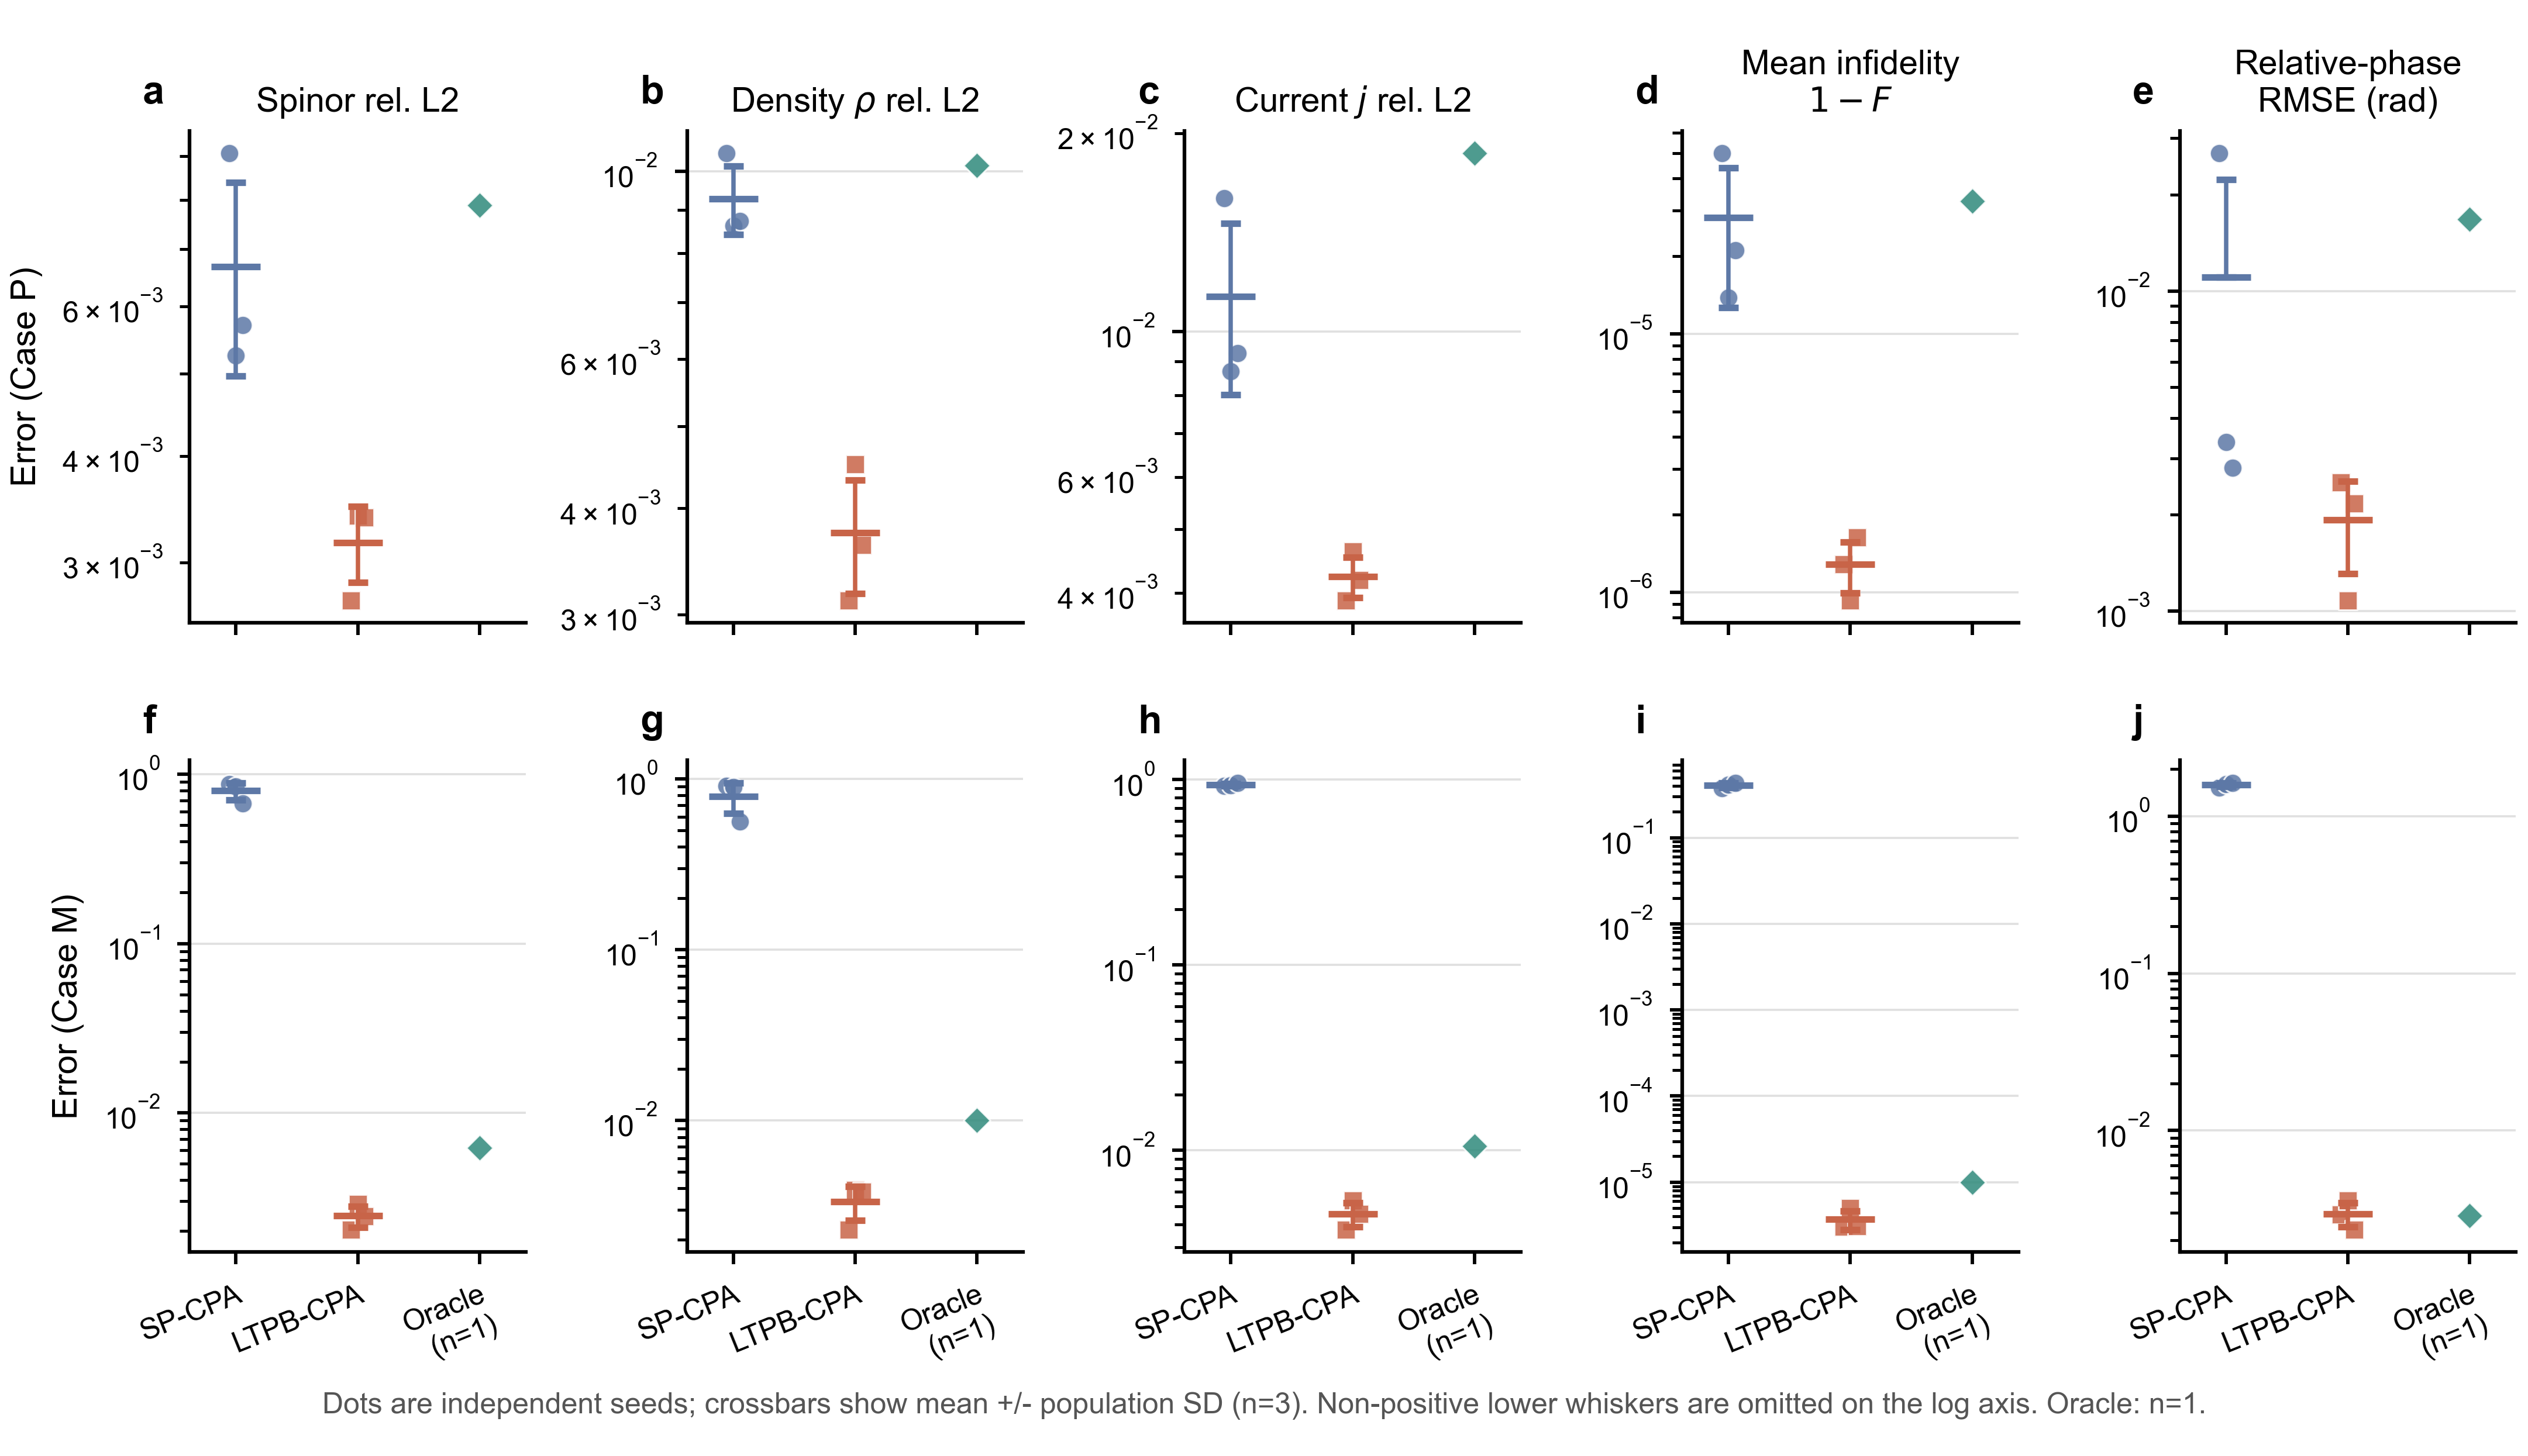
\includegraphics[width=0.88\textwidth]{results/figures/learned_two_phase_pilot/01_main_metric_comparison.png}
\caption{LTPB 未使用精确频率先验，并在纯能谱态与混合能谱态上均获得较低误差。}
\label{fig:ltpb-main}
\end{figure}

\begin{figure}[!htbp]
\centering
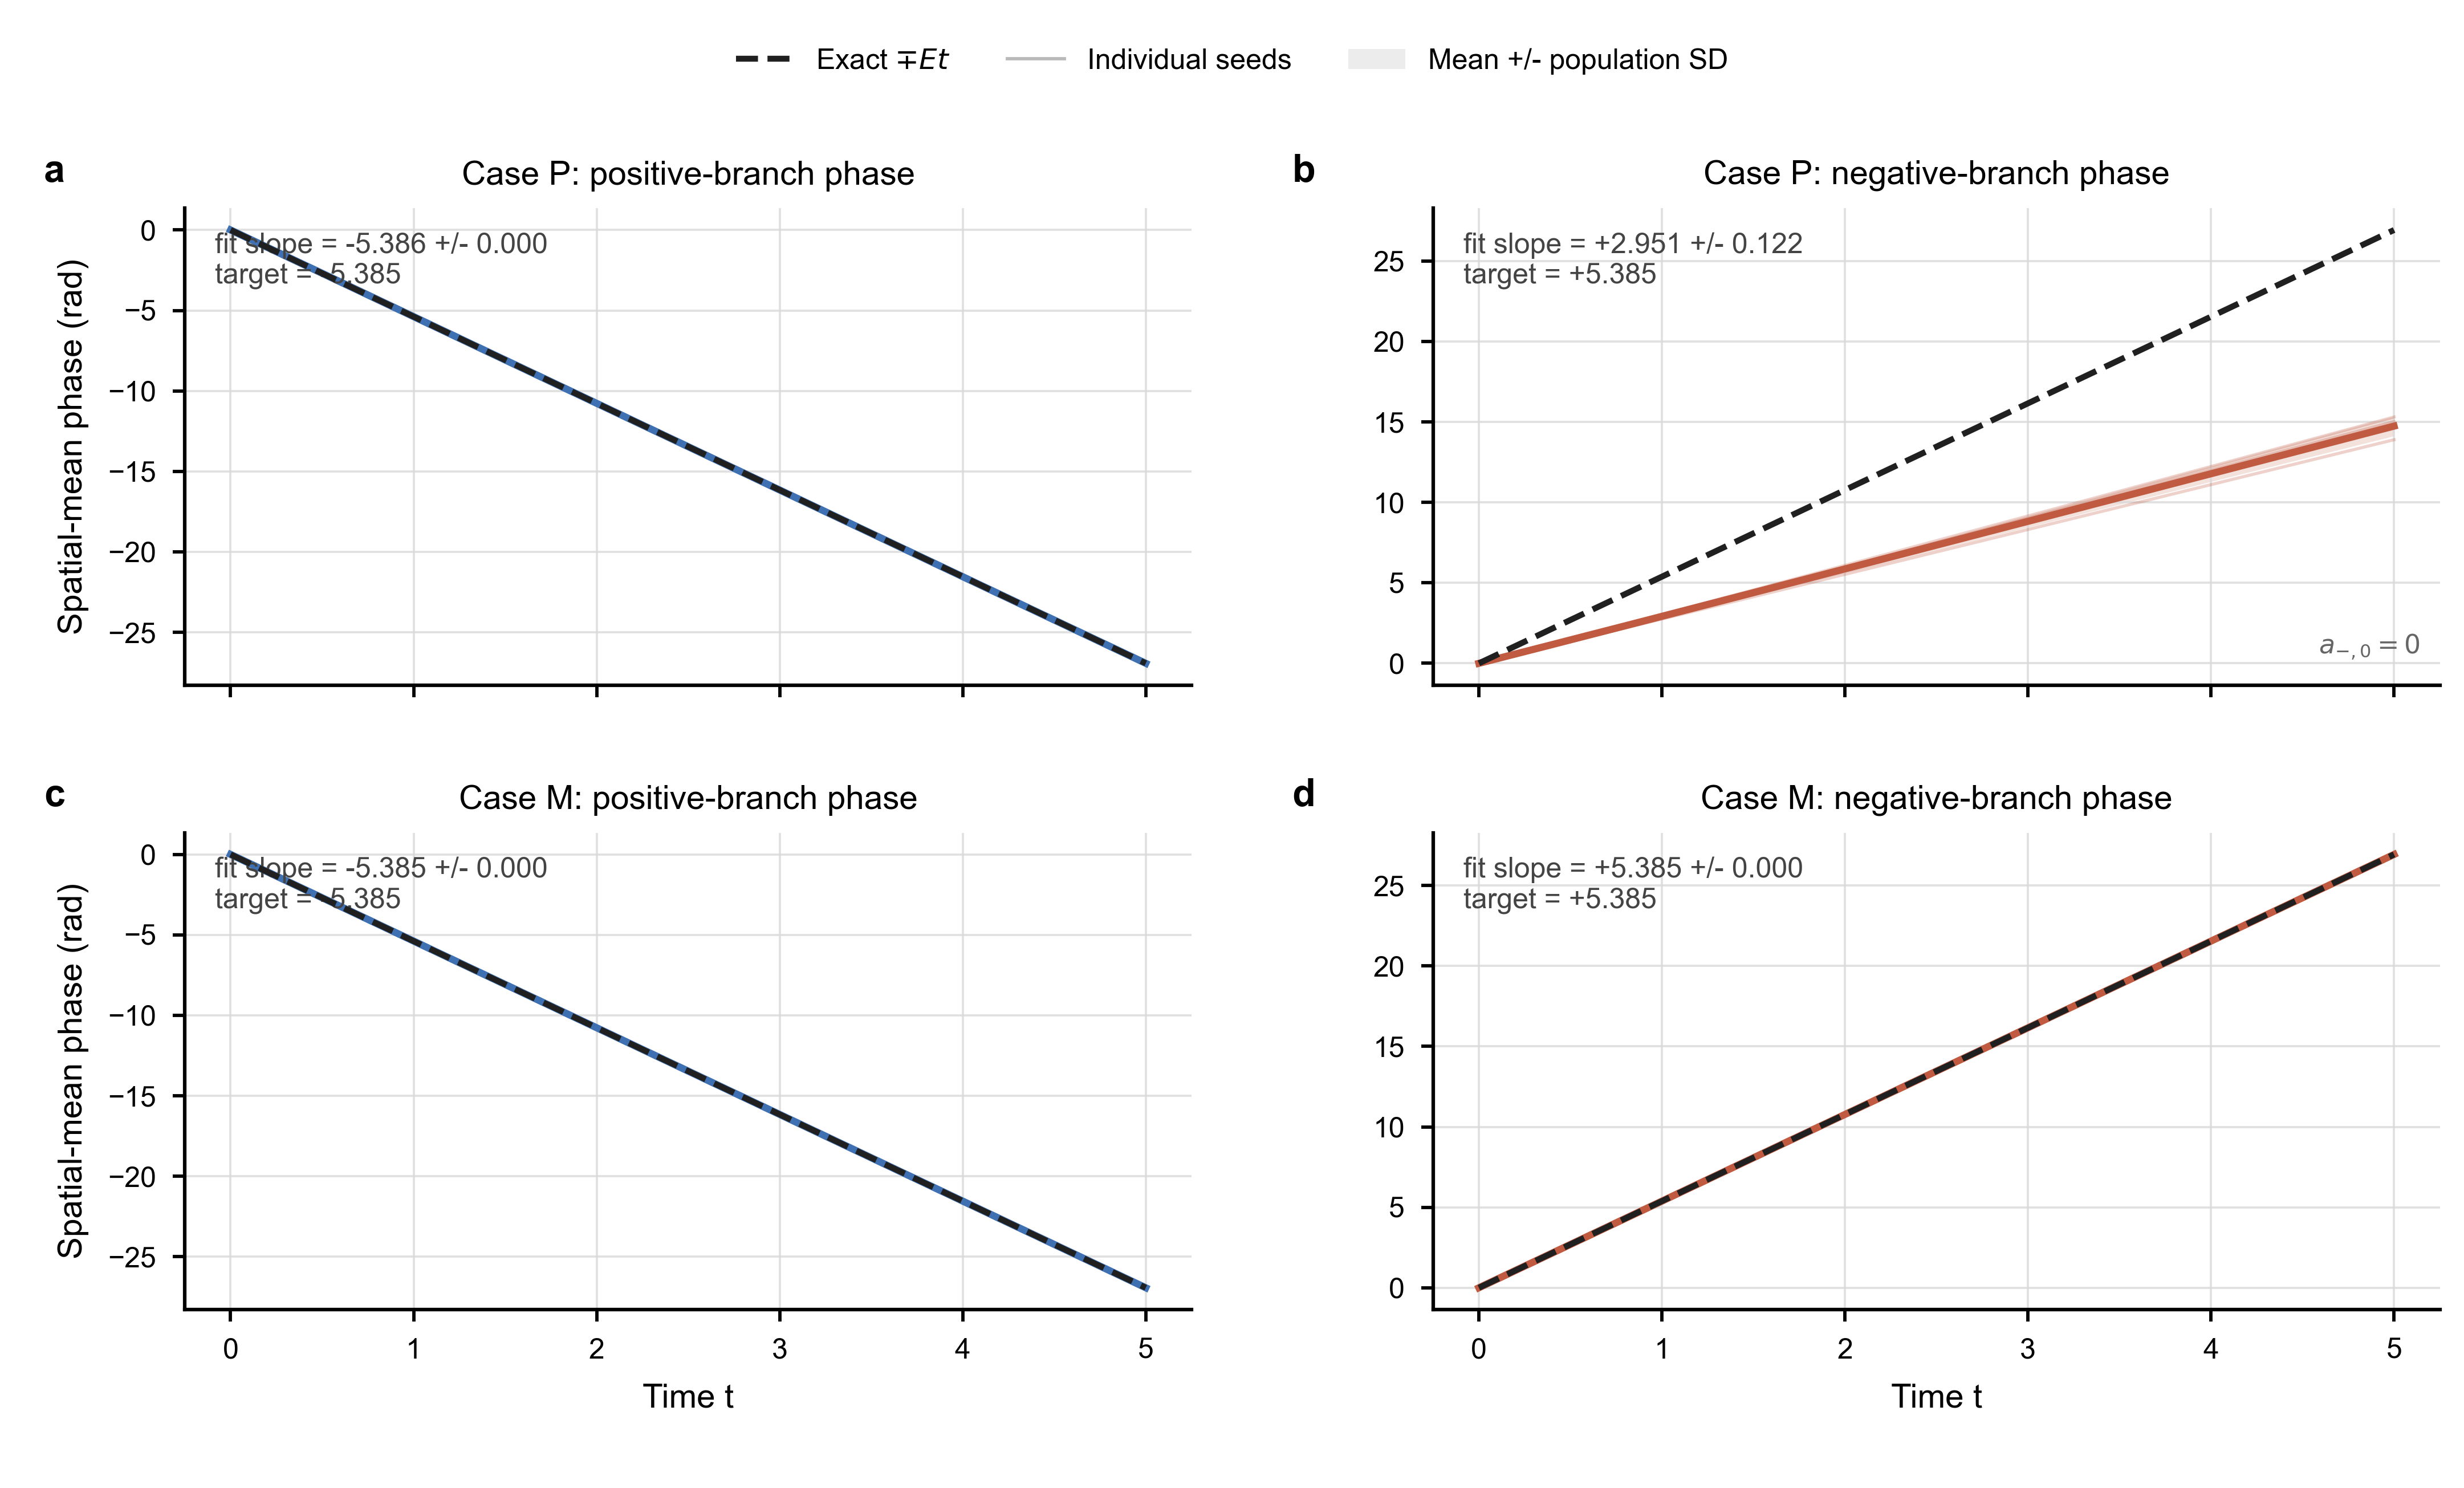
\includegraphics[width=0.88\textwidth]{results/figures/learned_two_phase_pilot/02_learned_branch_phases.png}
\caption{由方程残差辨识得到的两支相位分别接近 $-E_kt$ 与 $+E_kt$。}
\label{fig:ltpb-phase}
\end{figure}

精确相位斜率为 $\mp 5.3851648$，网络辨识结果为 $-5.3855$ 与 $+5.3854$；线性拟合的 $R^2$ 接近 1，振幅相对漂移低于 $0.3\%$。

\noindent\textbf{阶段结论：}
按能谱支分别设置相位函数后，支间相对相位及其对应的概率流振荡均得到准确恢复。

\section{阶段四：关键结构消融}

\subsection{消融设计}

五个模型均为 12996 左右参数，并使用配对初始化和配点序列。

\begin{table}[htbp]
\centering
\caption{关键结构消融设计}
\begin{tabular}{@{}lcc@{}}
\toprule
模型 & 能谱支对齐 & 独立振幅/相位 \\
\midrule
LTPB & 是 & 是 \\
BranchComplex & 是 & 否 \\
ComponentPolar & 否 & 是 \\
Rotated LTPB $15^\circ$ & 部分破坏 & 是 \\
Rotated LTPB $30^\circ$ & 进一步破坏 & 是 \\
\bottomrule
\end{tabular}
\end{table}

\subsection{结果}

\begin{table}[htbp]
\centering
\caption{关键结构消融结果}
\begin{tabular}{@{}lrrr@{}}
\toprule
模型 & 波函数误差 & 流密度误差 & 相对相位均方根误差 \\
\midrule
LTPB & \textbf{0.0025} & \textbf{0.0045} & \textbf{0.0029} \\
BranchComplex & 0.9014 & 0.9342 & 1.6268 \\
ComponentPolar & 0.8907 & 0.9309 & 1.4802 \\
Rotated LTPB $15^\circ$ & 0.8996 & 0.9426 & 1.5579 \\
Rotated LTPB $30^\circ$ & 0.9306 & 0.9590 & 1.6830 \\
\bottomrule
\end{tabular}
\end{table}

\begin{figure}[!htbp]
\centering
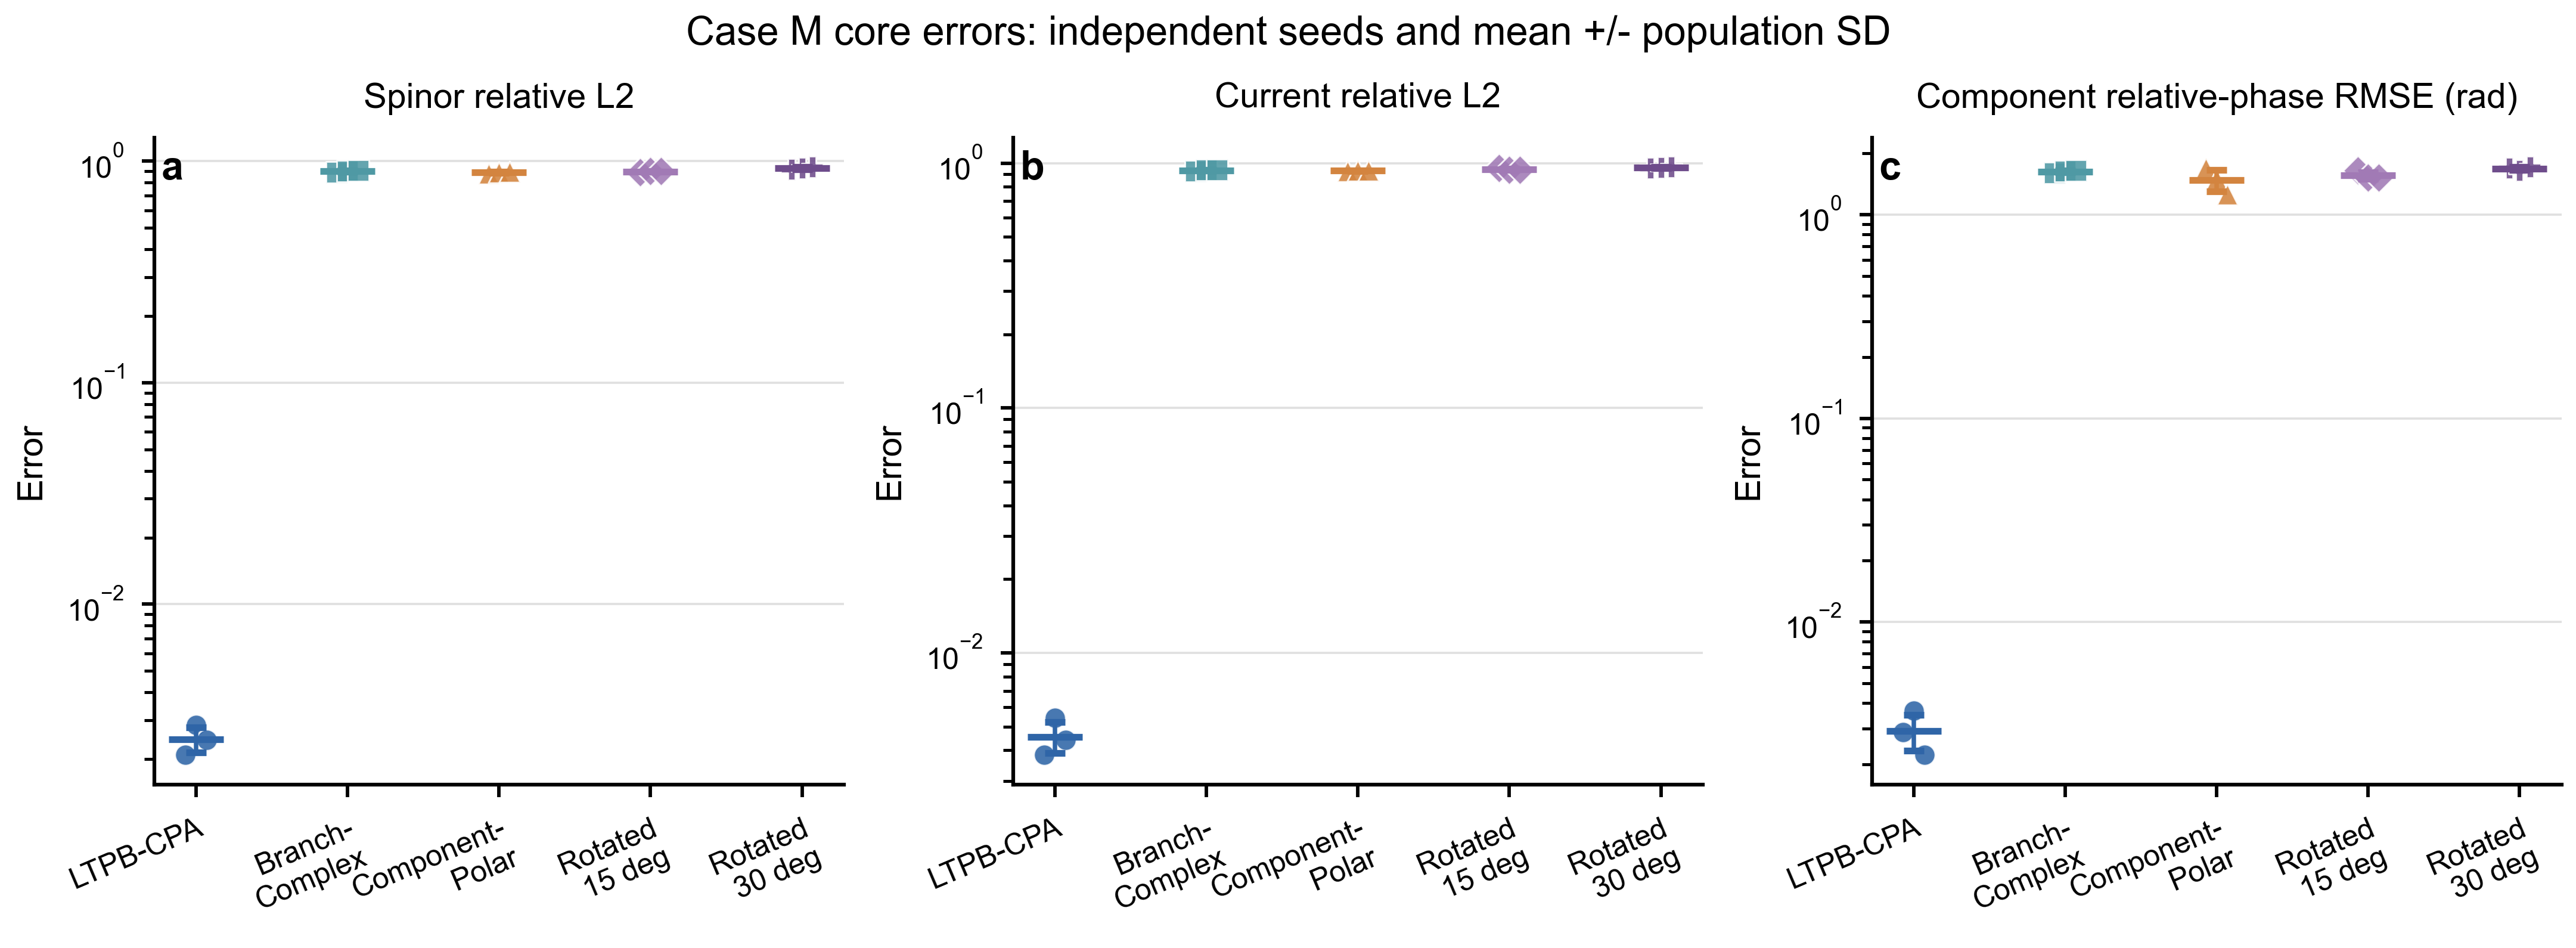
\includegraphics[width=0.88\textwidth]{results/figures/ltpb_mechanism_ablation/01_core_error_comparison.png}
\caption{单独采用能谱支基底或一般极坐标表示时，所得精度均低于完整 LTPB。}
\label{fig:ablation-core}
\end{figure}

\begin{figure}[!htbp]
\centering
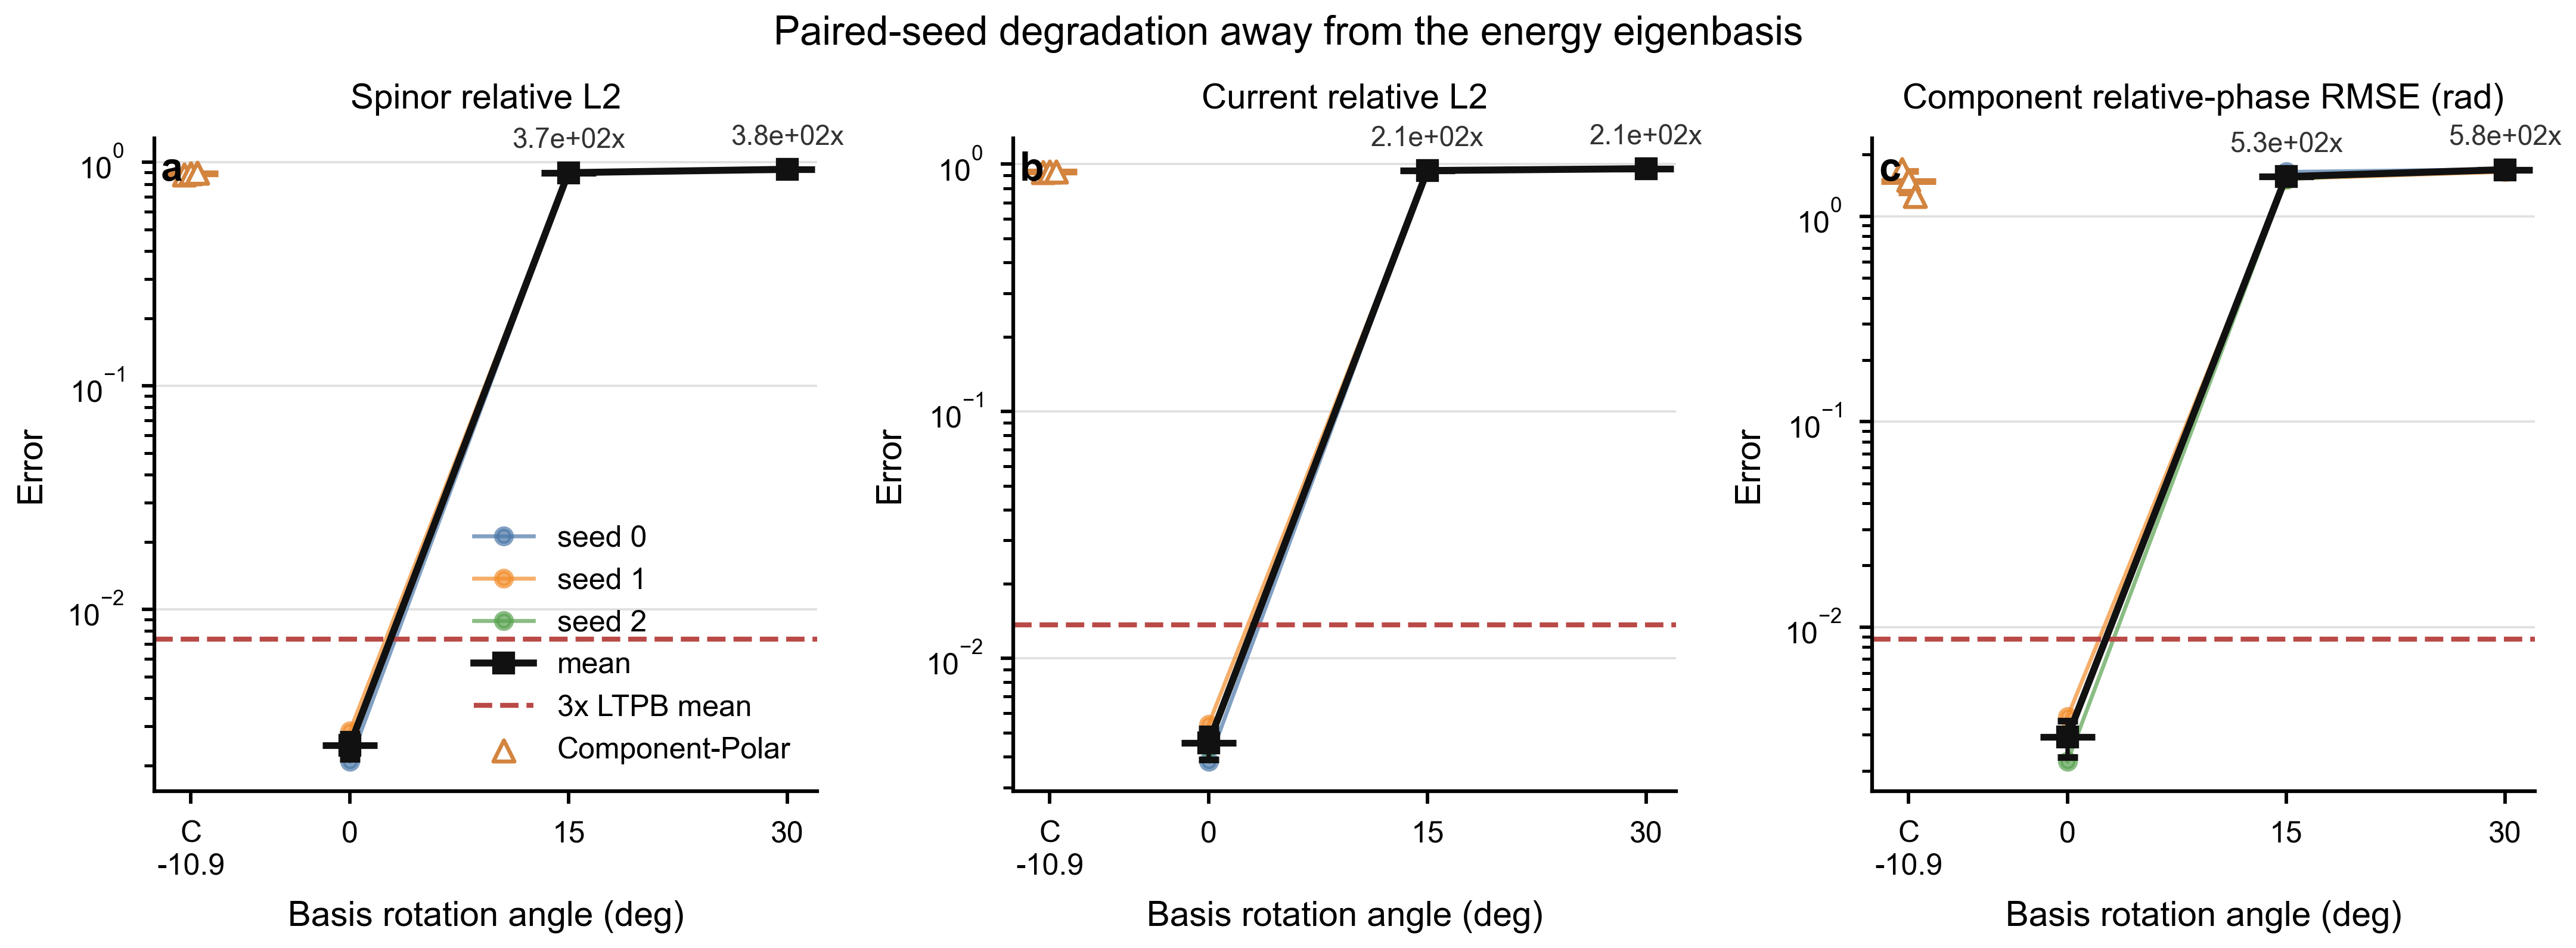
\includegraphics[width=0.88\textwidth]{results/figures/ltpb_mechanism_ablation/05_rotation_degradation.png}
\caption{能谱支基底发生旋转后，误差迅速进入接近单位相对误差的高值平台。}
\label{fig:ablation-rotation}
\end{figure}

预注册判据要求基底每增加一级旋转时误差至少增大 1.25 倍。实验中，模型在 $15^\circ$ 旋转时已进入高误差平台，$15^\circ\to30^\circ$ 仅继续增加约 $1.02$--$1.08$ 倍，因而该强判据未获满足。现有数据支持以下限于当前基准的结论：能谱支对齐与逐支相位表示均为获得低误差的必要结构条件。

\noindent\textbf{阶段结论：}
等参数消融排除了单纯增加参数规模和采用一般极坐标表示作为充分解释；低误差与能谱支对齐、逐支相位表示的联合结构相联系。由于旋转退化的强判据未获满足，机制归因仍限于当前自由单模基准。

\section{阶段五：双波数四能谱分量推广}

\subsection{问题与方法}

取 $k_1=2$、$k_2=5$，构造
\begin{equation}
\psi=\frac{1}{2\sqrt L}\sum_{l=1}^2
\left[
u_+(k_l)e^{ik_lx-iE_lt}
+u_-(k_l)e^{ik_lx+iE_lt}
\right].
\end{equation}
Multi-LTPB 为四个 $(k_l,\pm)$ 能谱通道分别设置可学习相位，训练过程中不使用精确能量 $E_l$。五个可训练模型采用近似相同的参数规模、5000 步优化及 5 个配对随机种子。

\subsection{结果}

\begin{table}[htbp]
\centering
\caption{双波数四能谱分量实验结果}
\begin{tabular}{@{}lrrl@{}}
\toprule
指标 & Multi-LTPB & 最佳可训练对照模型 & 对照/LTPB \\
\midrule
旋量波函数误差 & \textbf{0.006594} & 0.939819 & 142.52 \\
概率流密度误差 & \textbf{0.010976} & 0.957364 & 87.22 \\
保真度 & \textbf{0.999965} & 0.3172 & -- \\
配对种子 & \textbf{5/5 通过} & -- & -- \\
\bottomrule
\end{tabular}
\end{table}

\begin{figure}[!htbp]
\centering
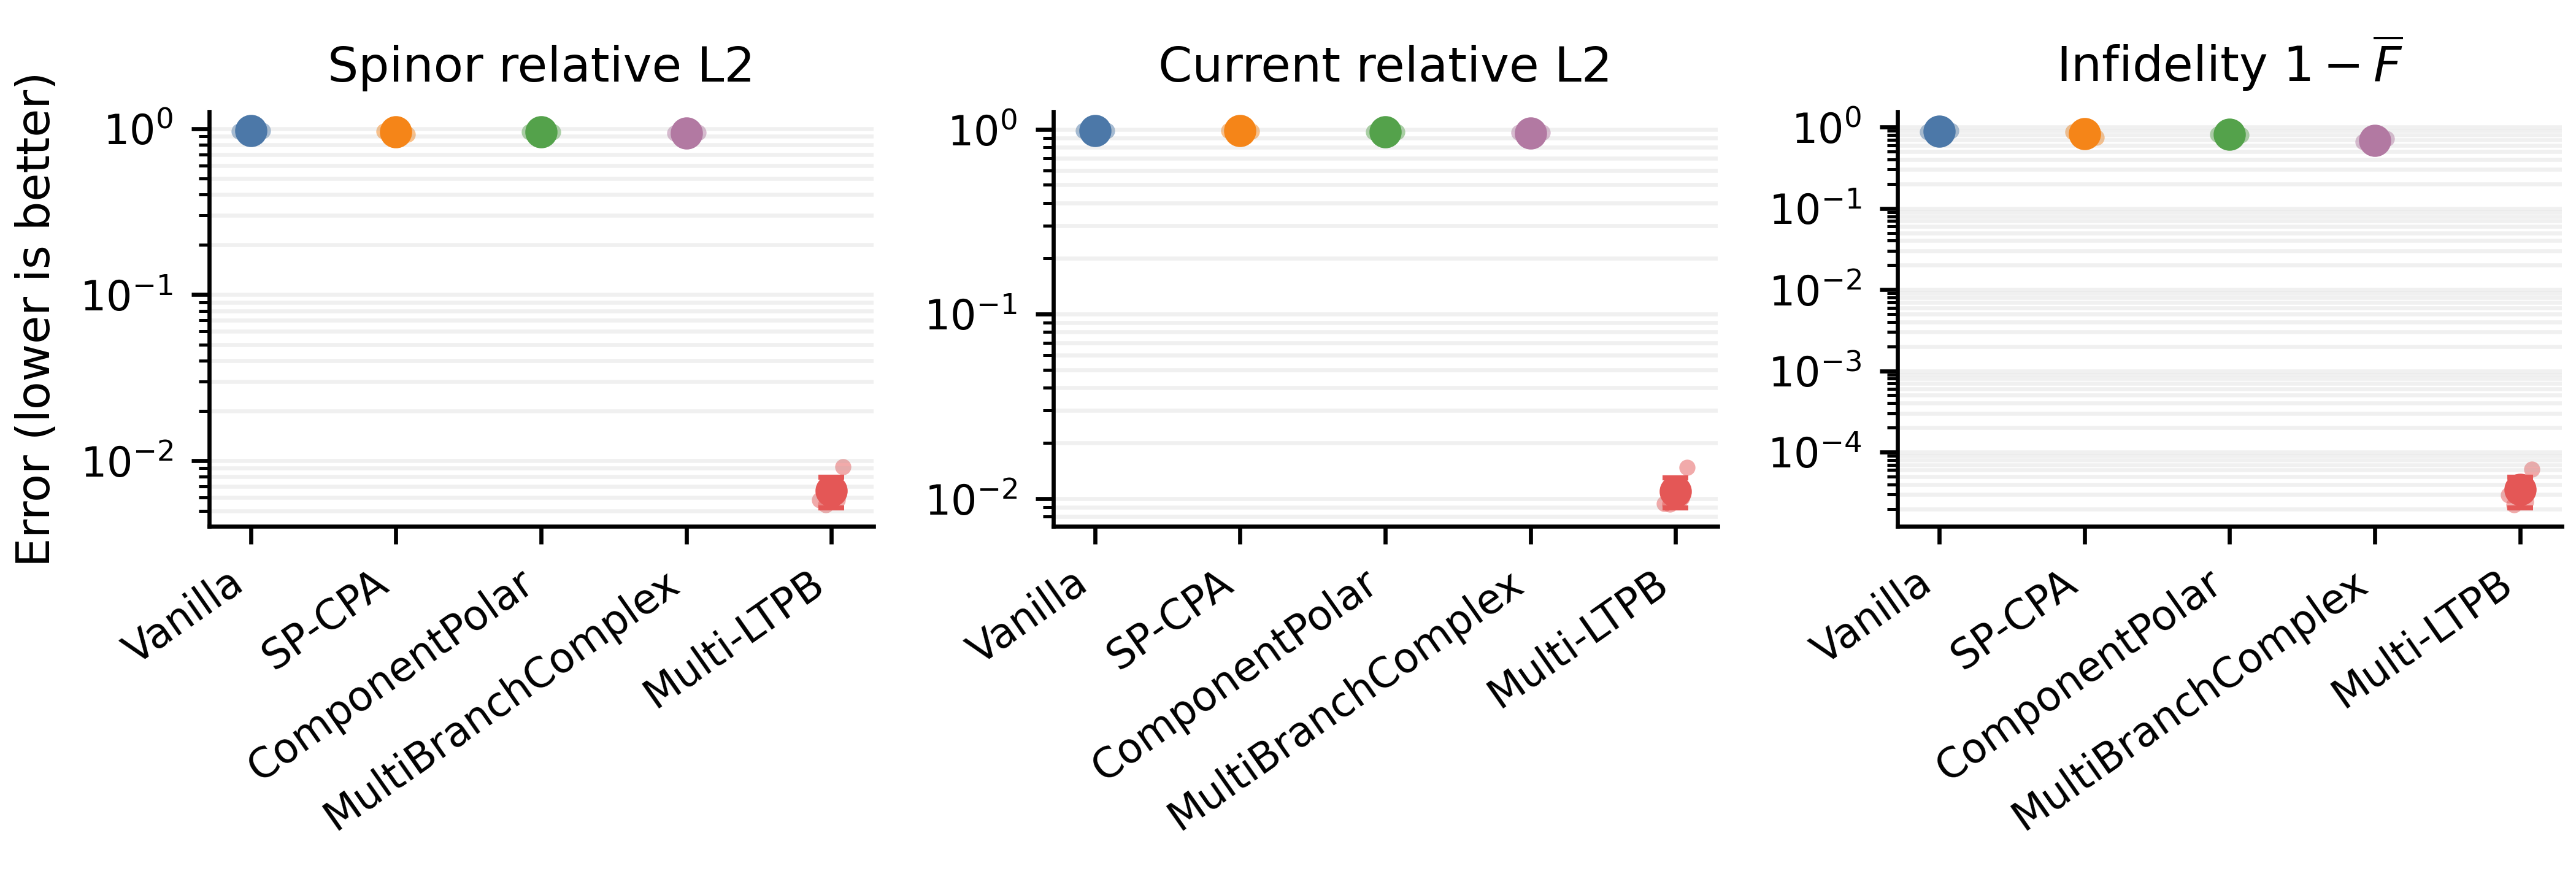
\includegraphics[width=0.88\textwidth]{results/figures/multimode_ltpb/primary_error_comparison.png}
\caption{Multi-LTPB 在两个波数、四个能谱分量的叠加态上保持较低误差。}
\label{fig:multi-error}
\end{figure}

\begin{figure}[!htbp]
\centering
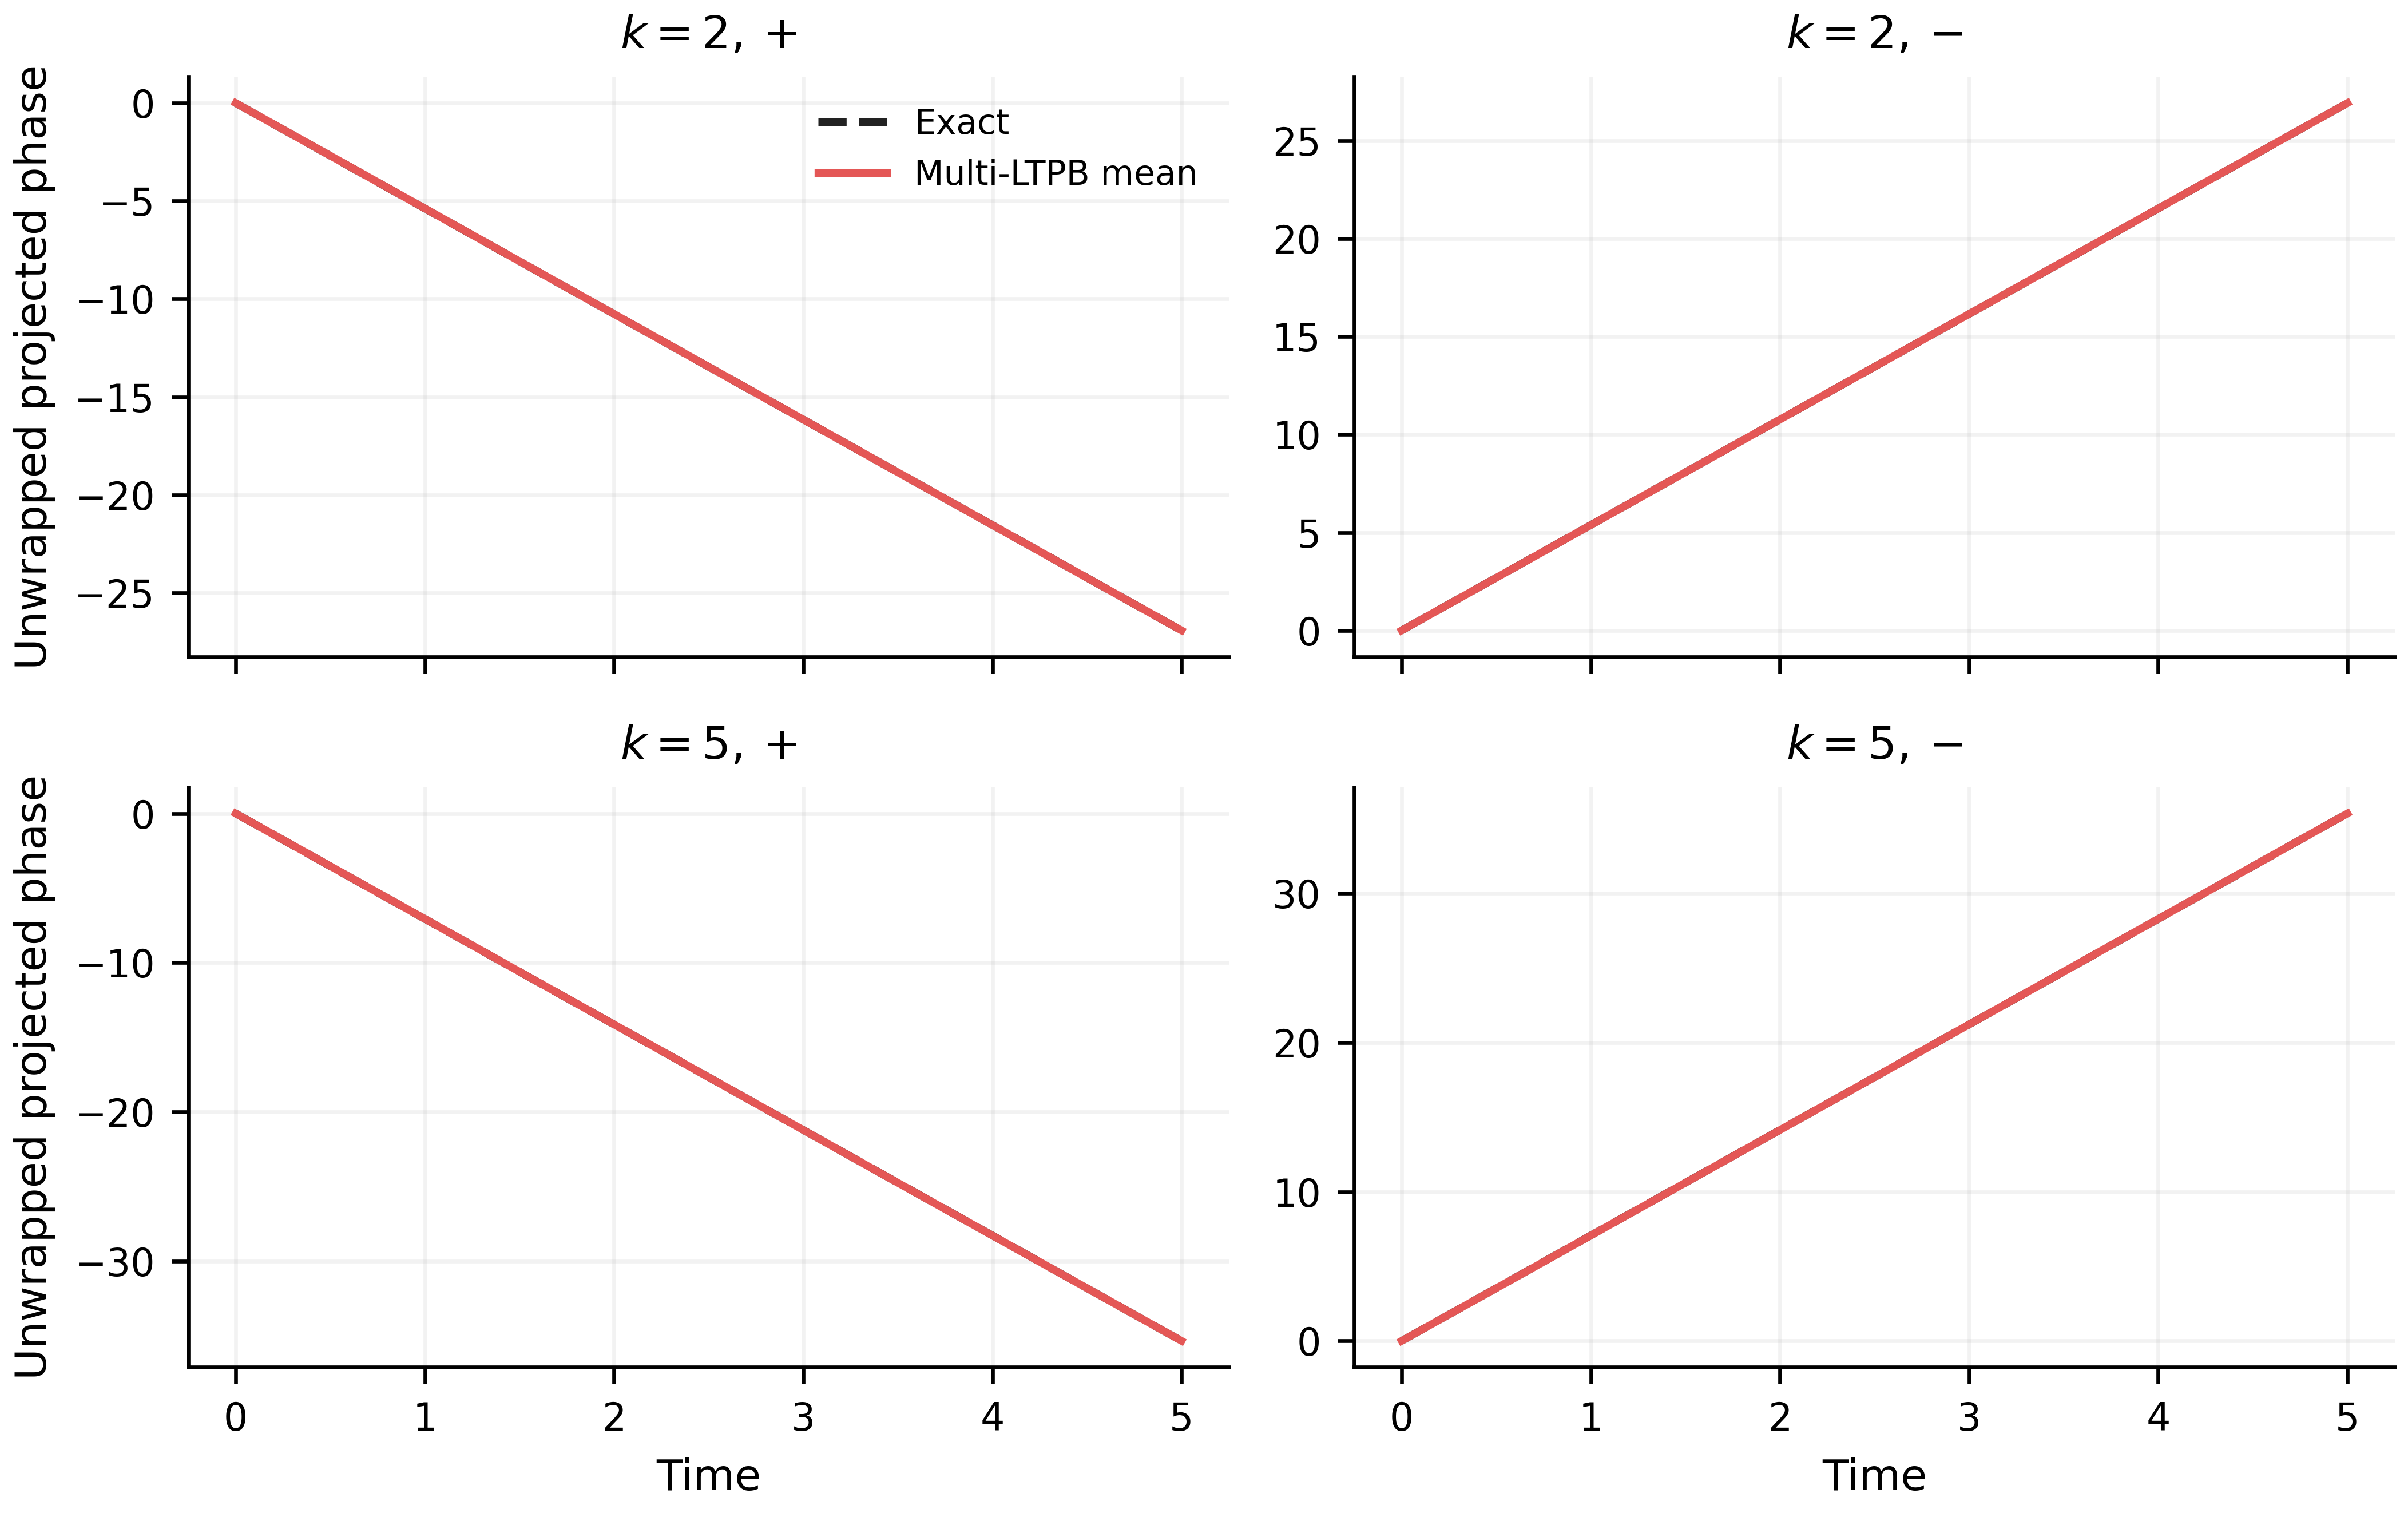
\includegraphics[width=0.88\textwidth]{results/figures/multimode_ltpb/learned_four_phases.png}
\caption{四个谱投影相位的斜率均与精确时间频率一致，平均相对误差约为 $0.03\%$。}
\label{fig:multi-phase}
\end{figure}

\begin{figure}[!htbp]
\centering
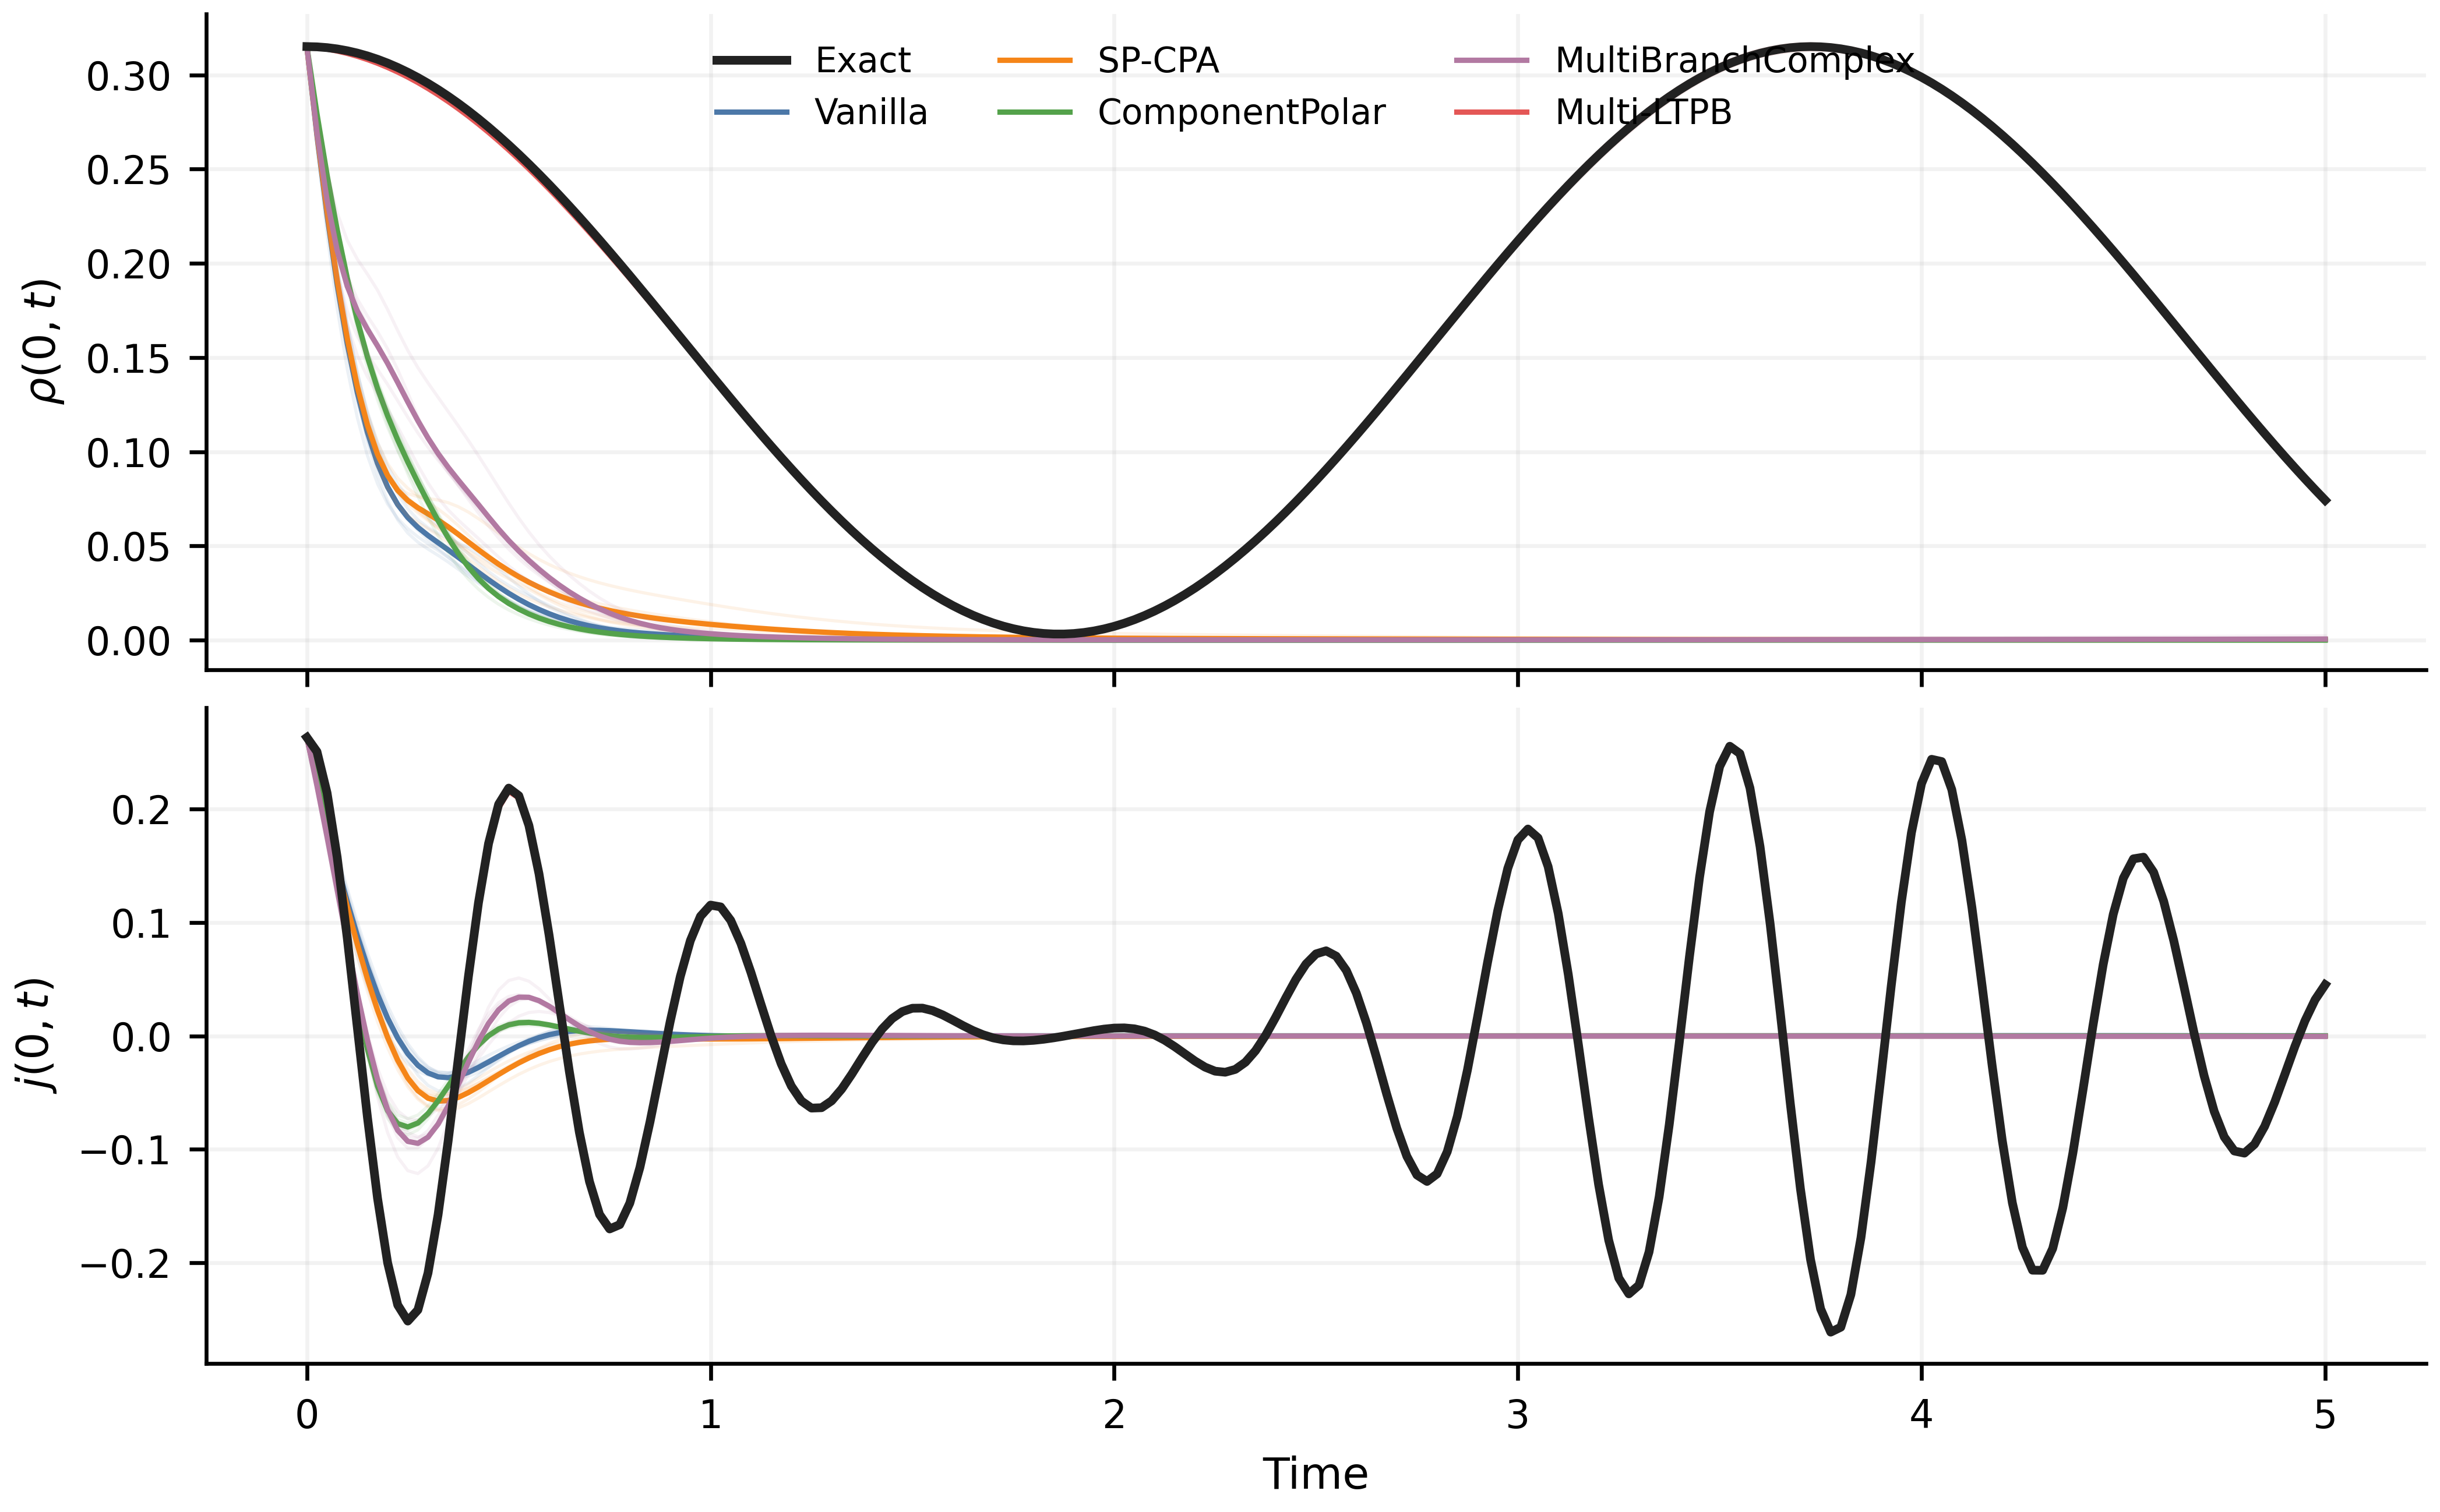
\includegraphics[width=0.88\textwidth]{results/figures/multimode_ltpb/representative_density_current.png}
\caption{模型恢复了不同空间模态及正、负能谱支共同产生的概率密度与概率流干涉。}
\label{fig:multi-current}
\end{figure}

\noindent\textbf{阶段结论：}
第五阶段满足全部预注册精度判据，表明逐支相位表示可扩展至多个已知的离散能谱分量。该结论依赖预先给定的波数集合及相应本征旋量基底。

\section{阶段六：连续高斯波包与共享谱 LTPB}

\subsection{问题}

在 $L=16\pi$、$m=5$、$T=5$ 上取 33 个波数 $k_n=n/8\in[0,4]$。初始动量分布为中心 $k_0=2$、宽度 $\sigma_k=0.5$ 的高斯谱，正、负能谱支等权叠加。由于演化同时包含数十个色散频率分量，逐个增加独立网络输出将使参数规模随模态数增长。

\subsection{共享谱方法}

使用一个共享网络接收 $(k,t)$，输出两支振幅和相位：
\begin{equation}
\widehat{\widetilde\psi}(k,t)=
a_+(k,t)u_+(k)e^{iS_+(k,t)}
+a_-(k,t)u_-(k)e^{iS_-(k,t)}.
\end{equation}
训练采用原旋量表象中的非对角谱残差
\begin{equation}
R_k=i\partial_t\widetilde\psi
-(k\sigma_x+m\sigma_z)\widetilde\psi,
\end{equation}
其中未引入精确色散关系 $E(k)$ 作为监督信息。对于自由周期问题，Parseval 恒等式保证该谱残差与对应的坐标空间残差等价。网络参数量保持为 12932，未随模态数作线性增加。

\subsection{结果}

\begin{table}[htbp]
\centering
\small
\caption{连续高斯波包实验结果}
\begin{tabularx}{\textwidth}{@{}Y r r l@{}}
\toprule
指标 & Shared-Spectral-LTPB & 最佳可训练对照模型 & 误差比或判据 \\
\midrule
旋量波函数误差 & \textbf{0.041038} & 0.909412 & 22.16 \\
密度误差 & \textbf{0.015262} & 0.487106 & -- \\
概率流密度误差 & \textbf{0.048057} & 0.884010 & 18.40 \\
保真度 & \textbf{0.998249} & 0.386112 & 满足判据 \\
配对种子 & \textbf{5/5 通过} & -- & 通过 \\
训练波数相位误差 & \textbf{0.115\%} & -- & $<1\%$ \\
未训练中点相位误差 & \textbf{0.115\%} & -- & $<2\%$ \\
\bottomrule
\end{tabularx}
\end{table}

\begin{figure}[!htbp]
\centering
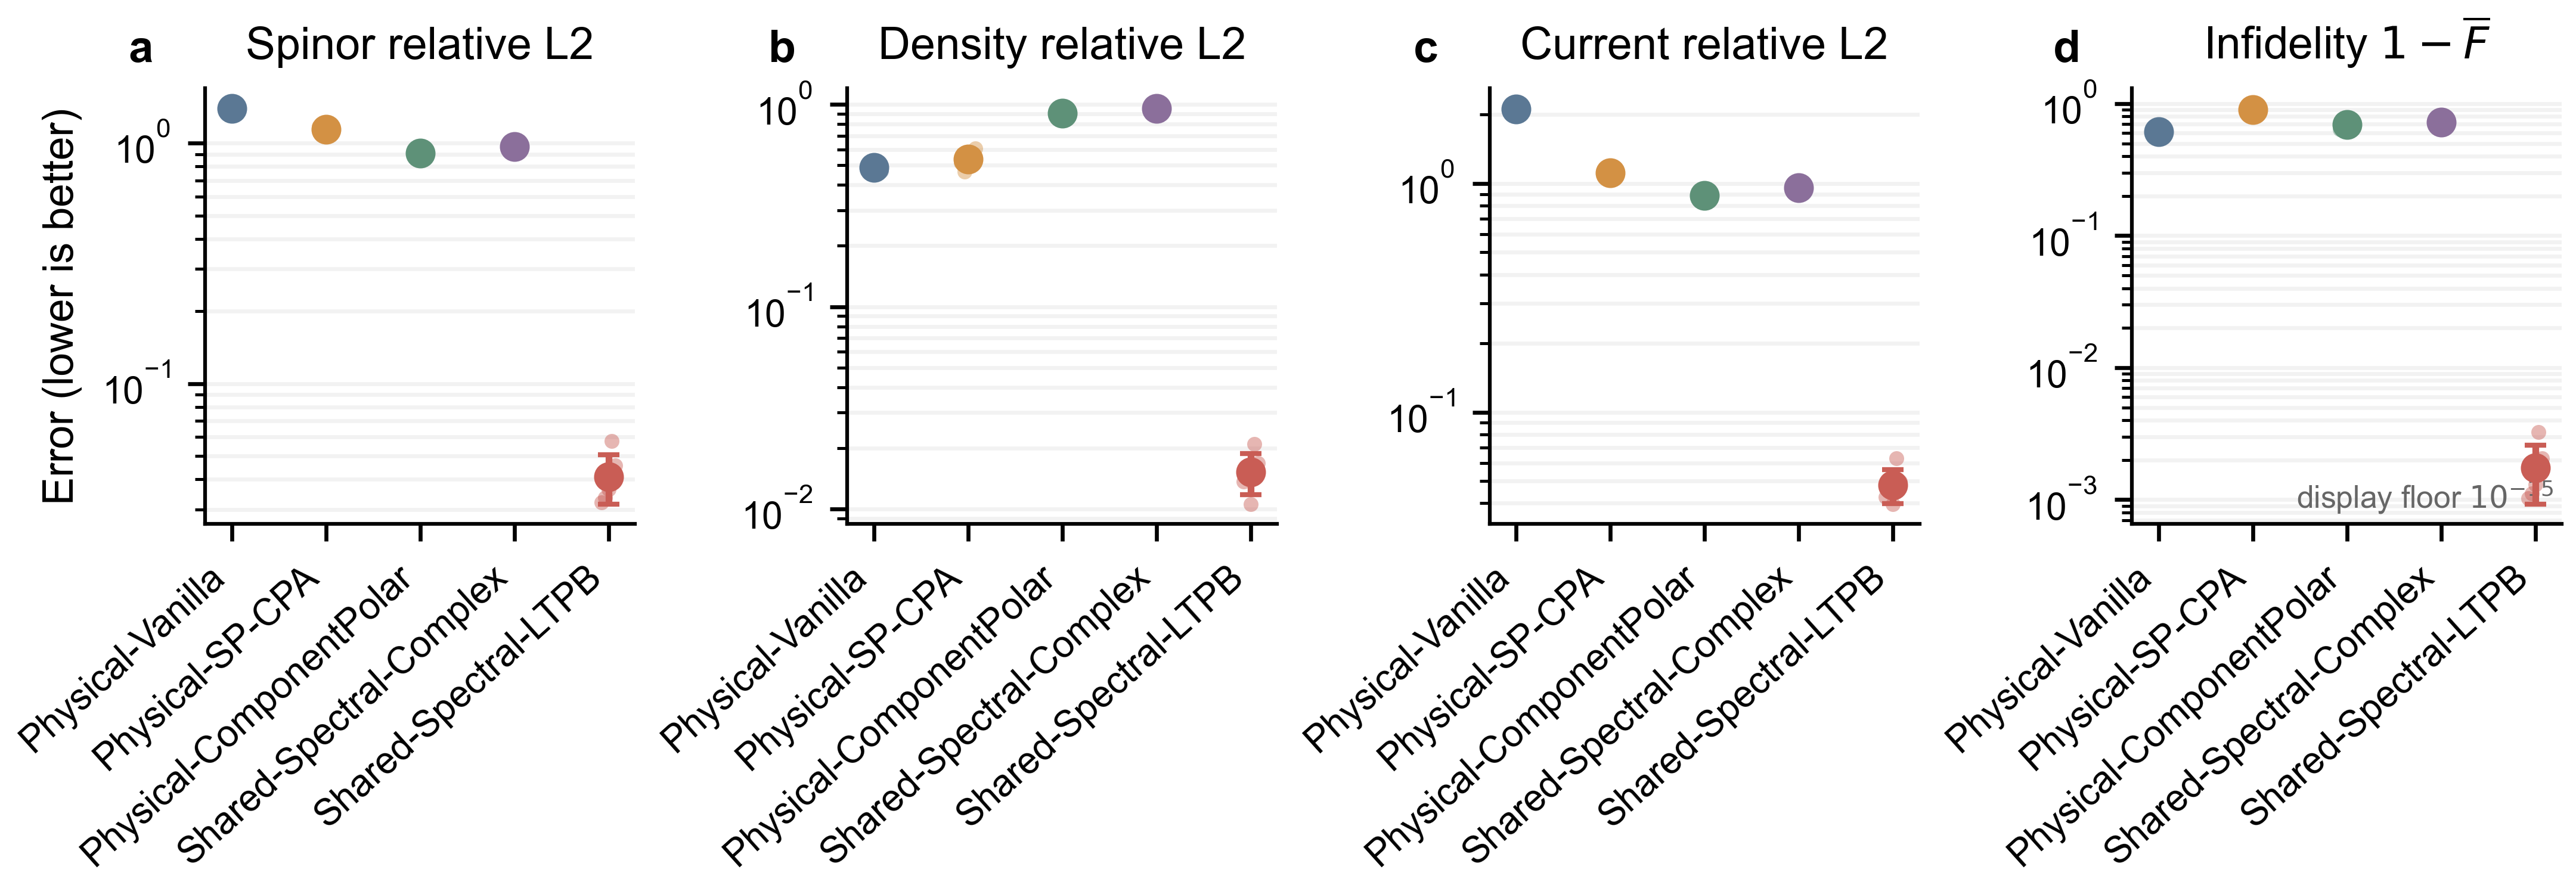
\includegraphics[width=0.88\textwidth]{results/figures/wavepacket_shared_spectral_ltpb/primary_error_comparison.png}
\caption{固定参数规模下，共享谱 LTPB 的误差低于坐标空间模型及同基底复系数模型。}
\label{fig:wavepacket-error}
\end{figure}

\begin{figure}[!htbp]
\centering
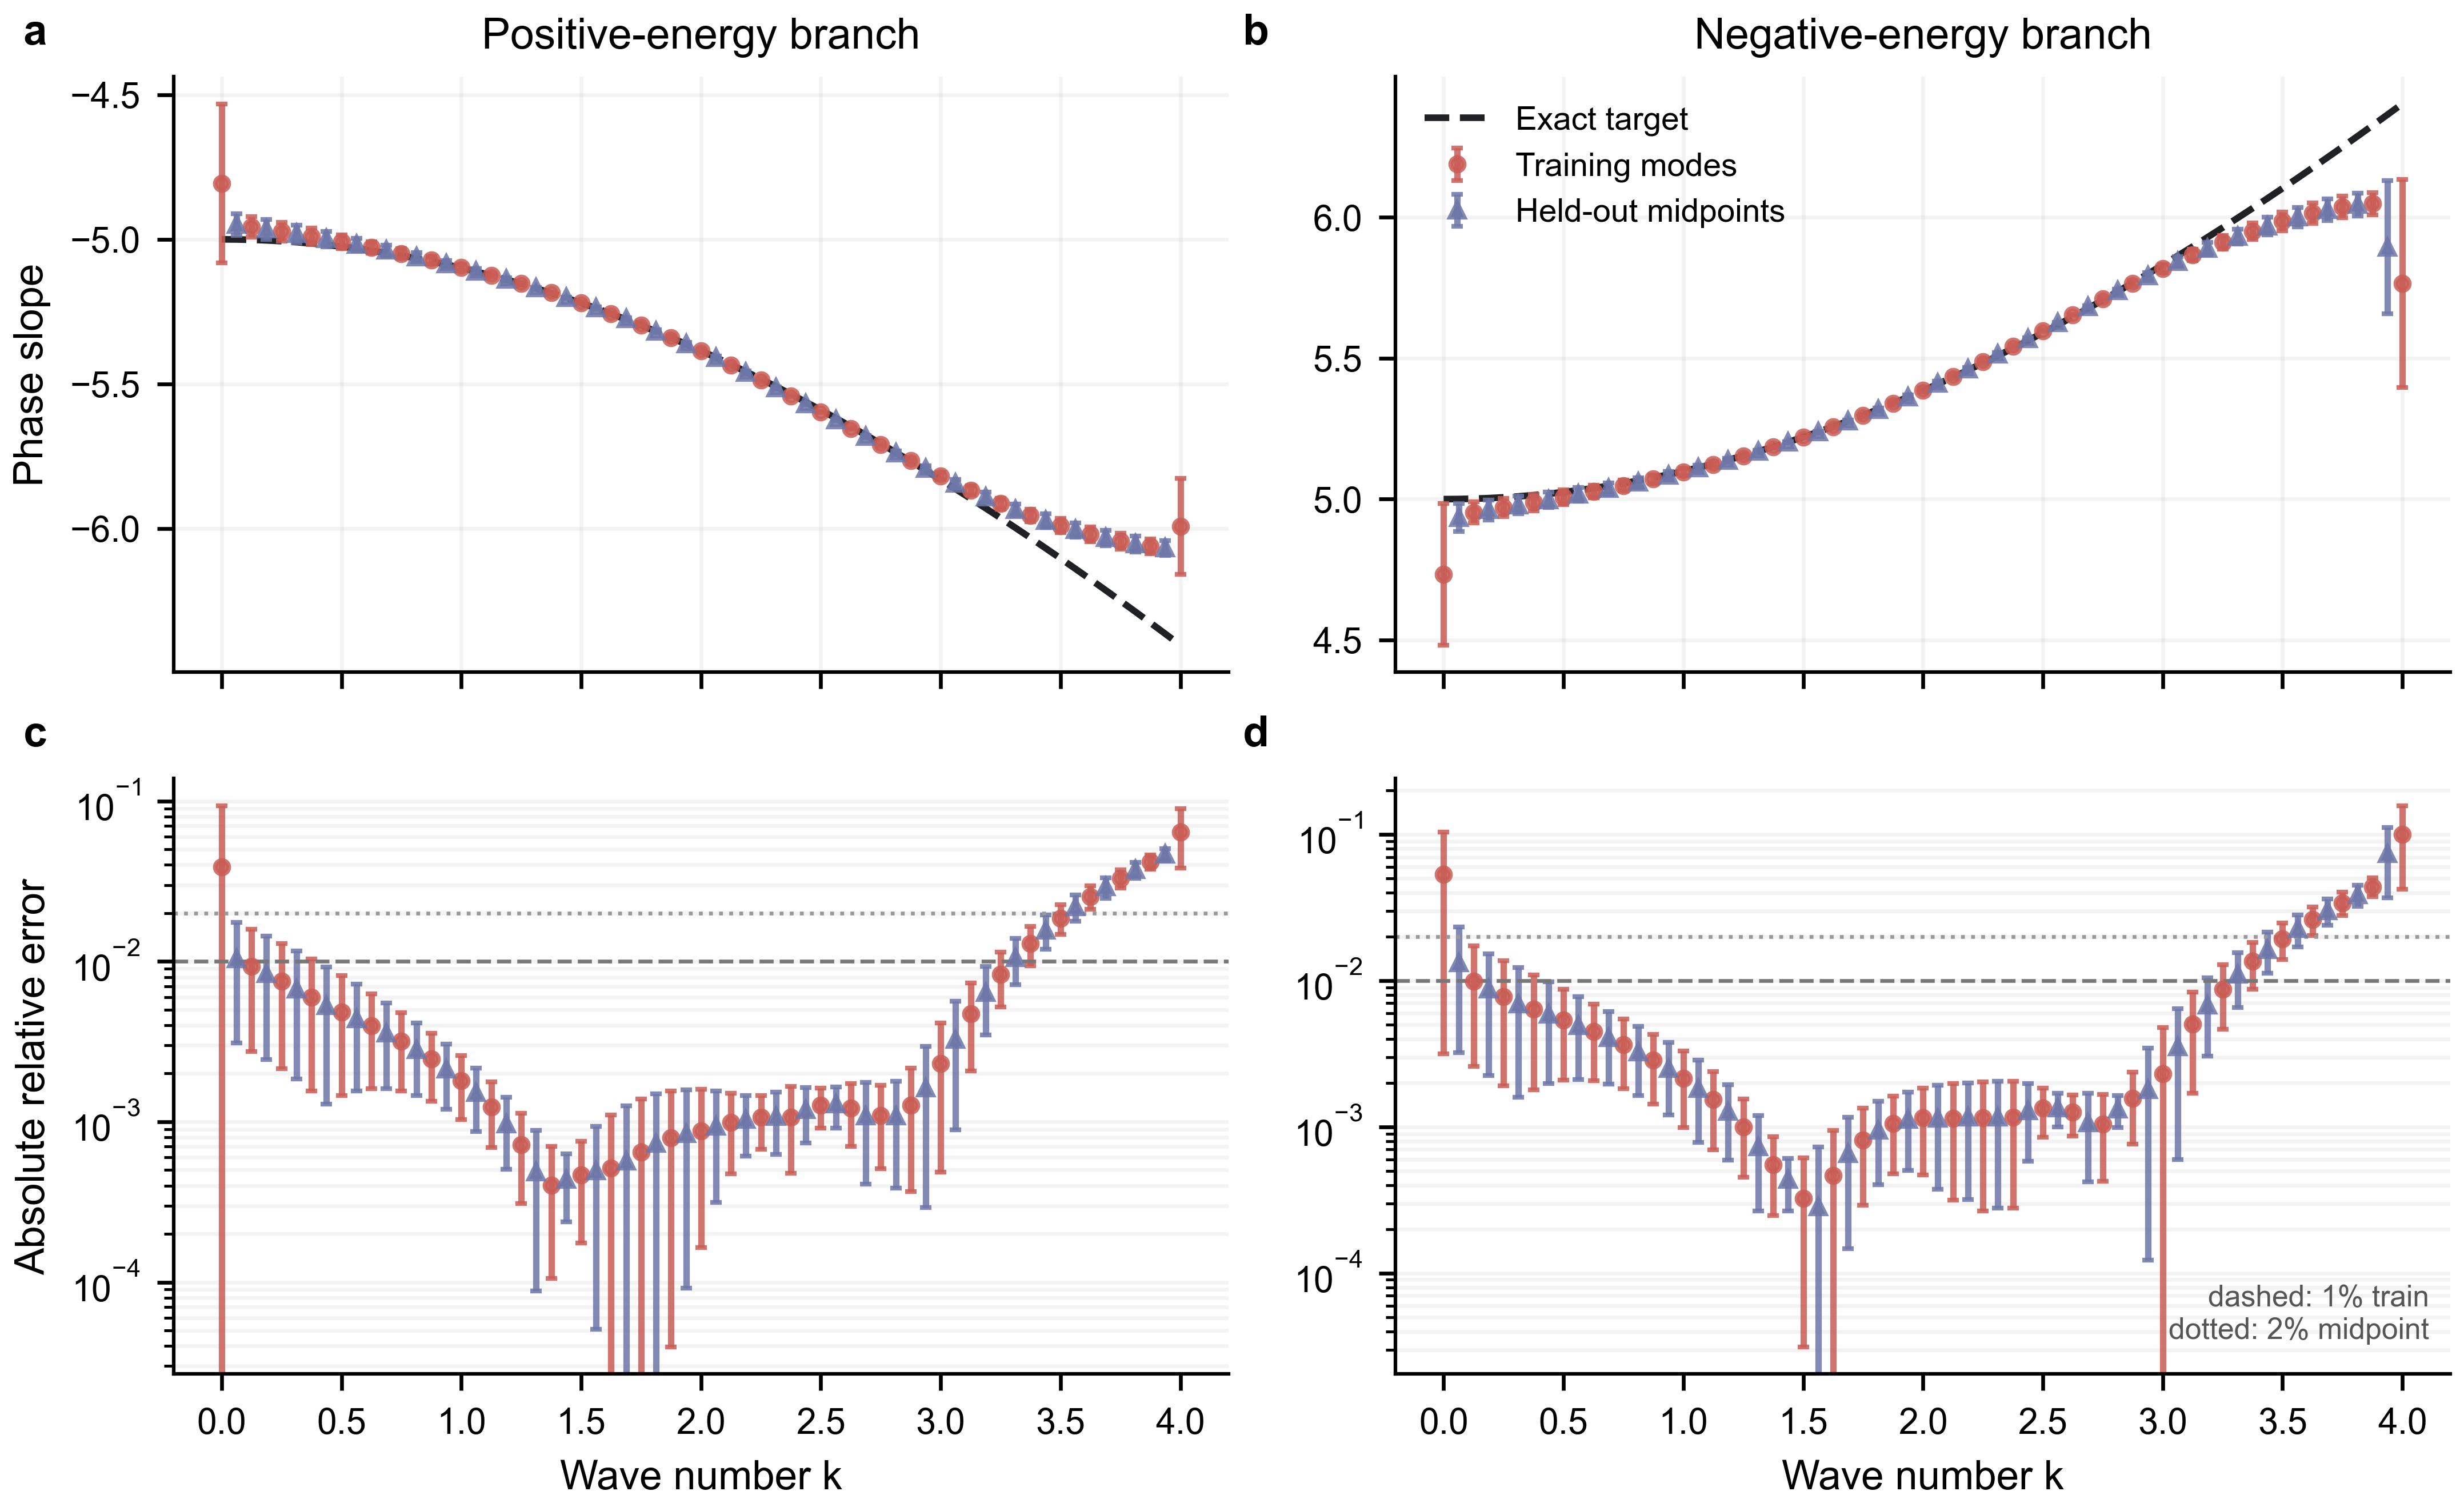
\includegraphics[width=0.88\textwidth]{results/figures/wavepacket_shared_spectral_ltpb/phase_slope_train_midpoint.png}
\caption{共享网络在未参与训练的波数中点处仍给出接近精确值的相位斜率。}
\label{fig:wavepacket-phase}
\end{figure}

\begin{figure}[!htbp]
\centering
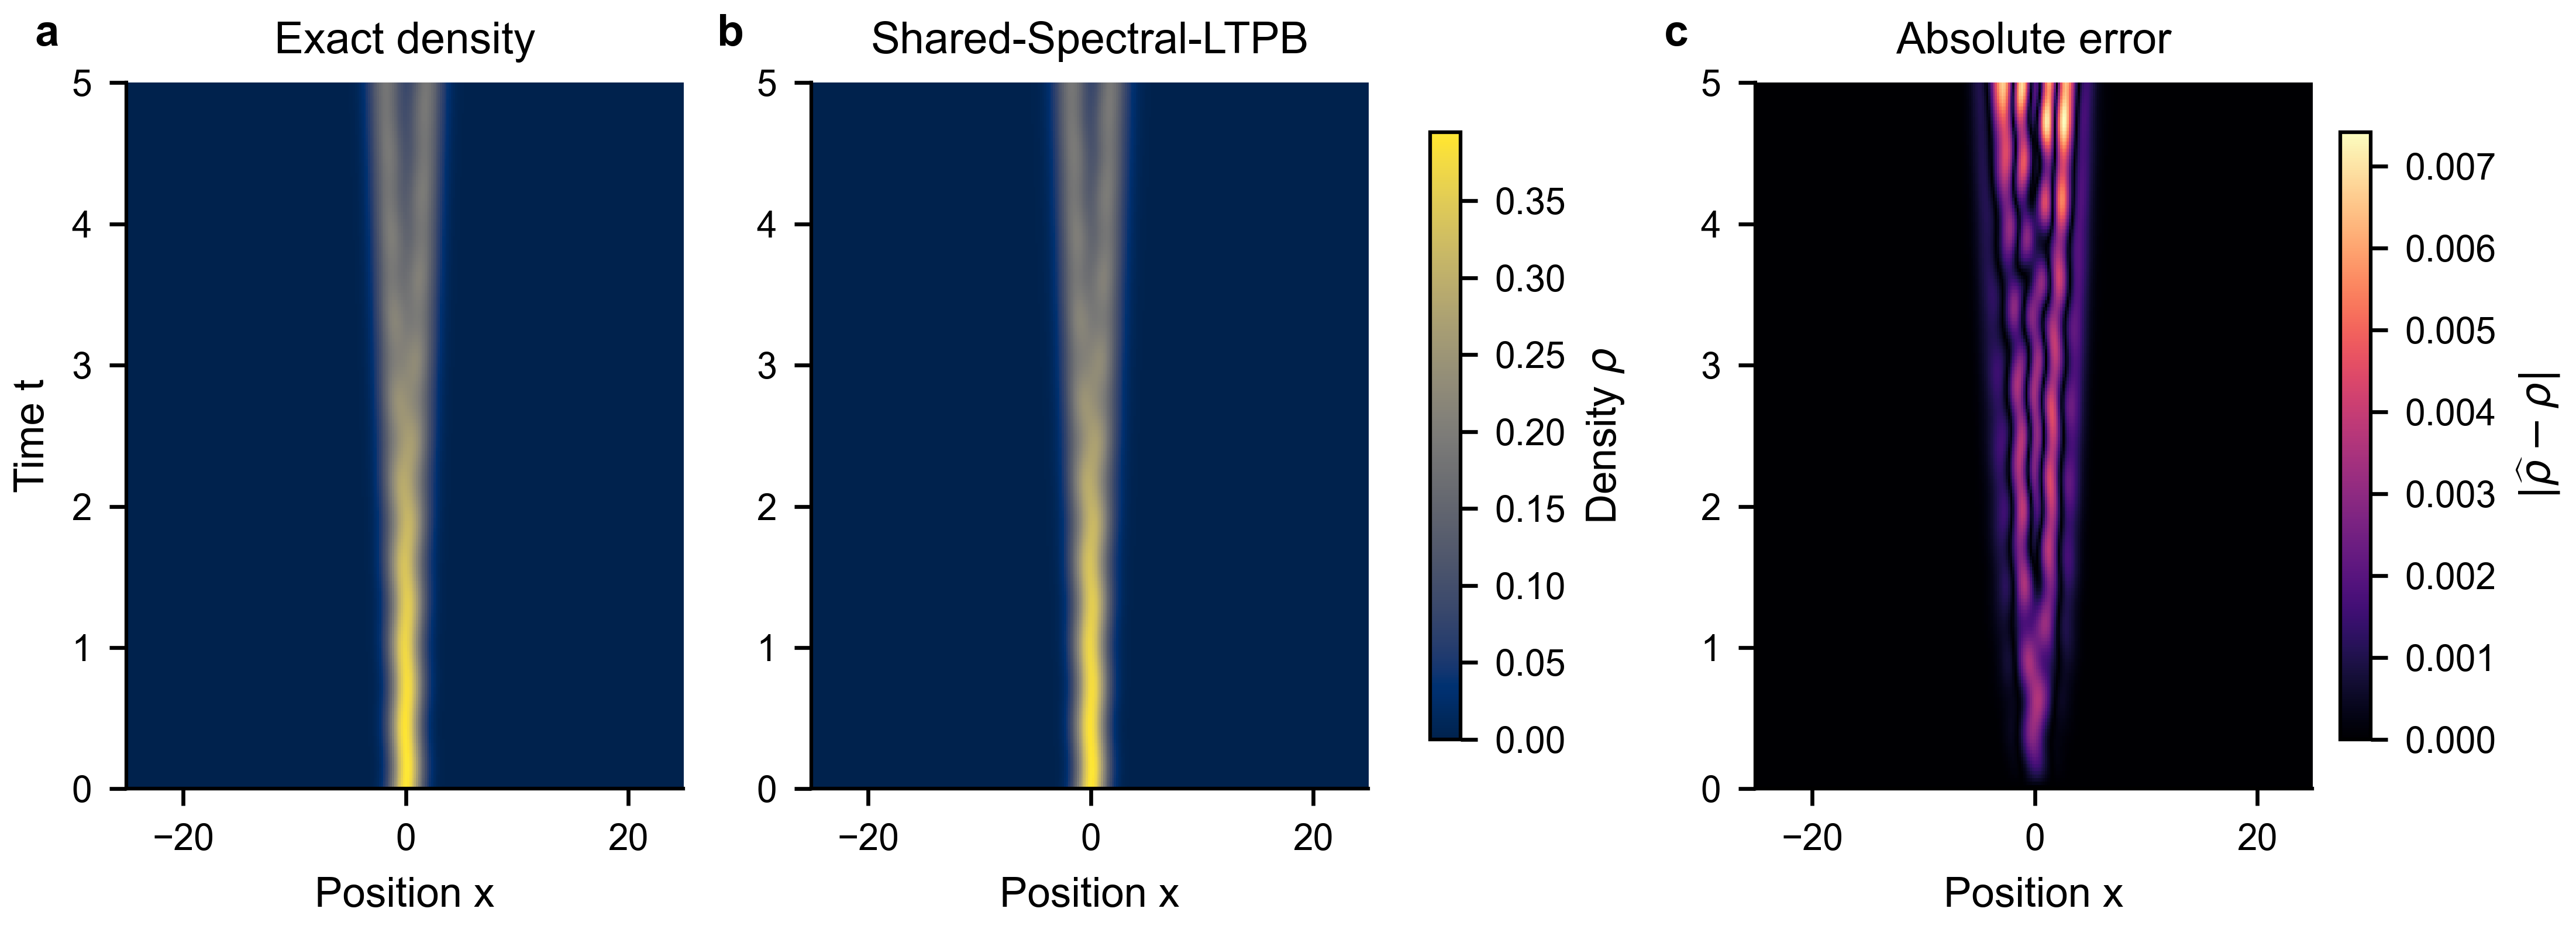
\includegraphics[width=0.88\textwidth]{results/figures/wavepacket_shared_spectral_ltpb/wavepacket_density_spacetime.png}
\caption{共享谱 LTPB 所得高斯波包概率密度及其绝对误差。}
\label{fig:wavepacket-density}
\end{figure}

\begin{figure}[!htbp]
\centering
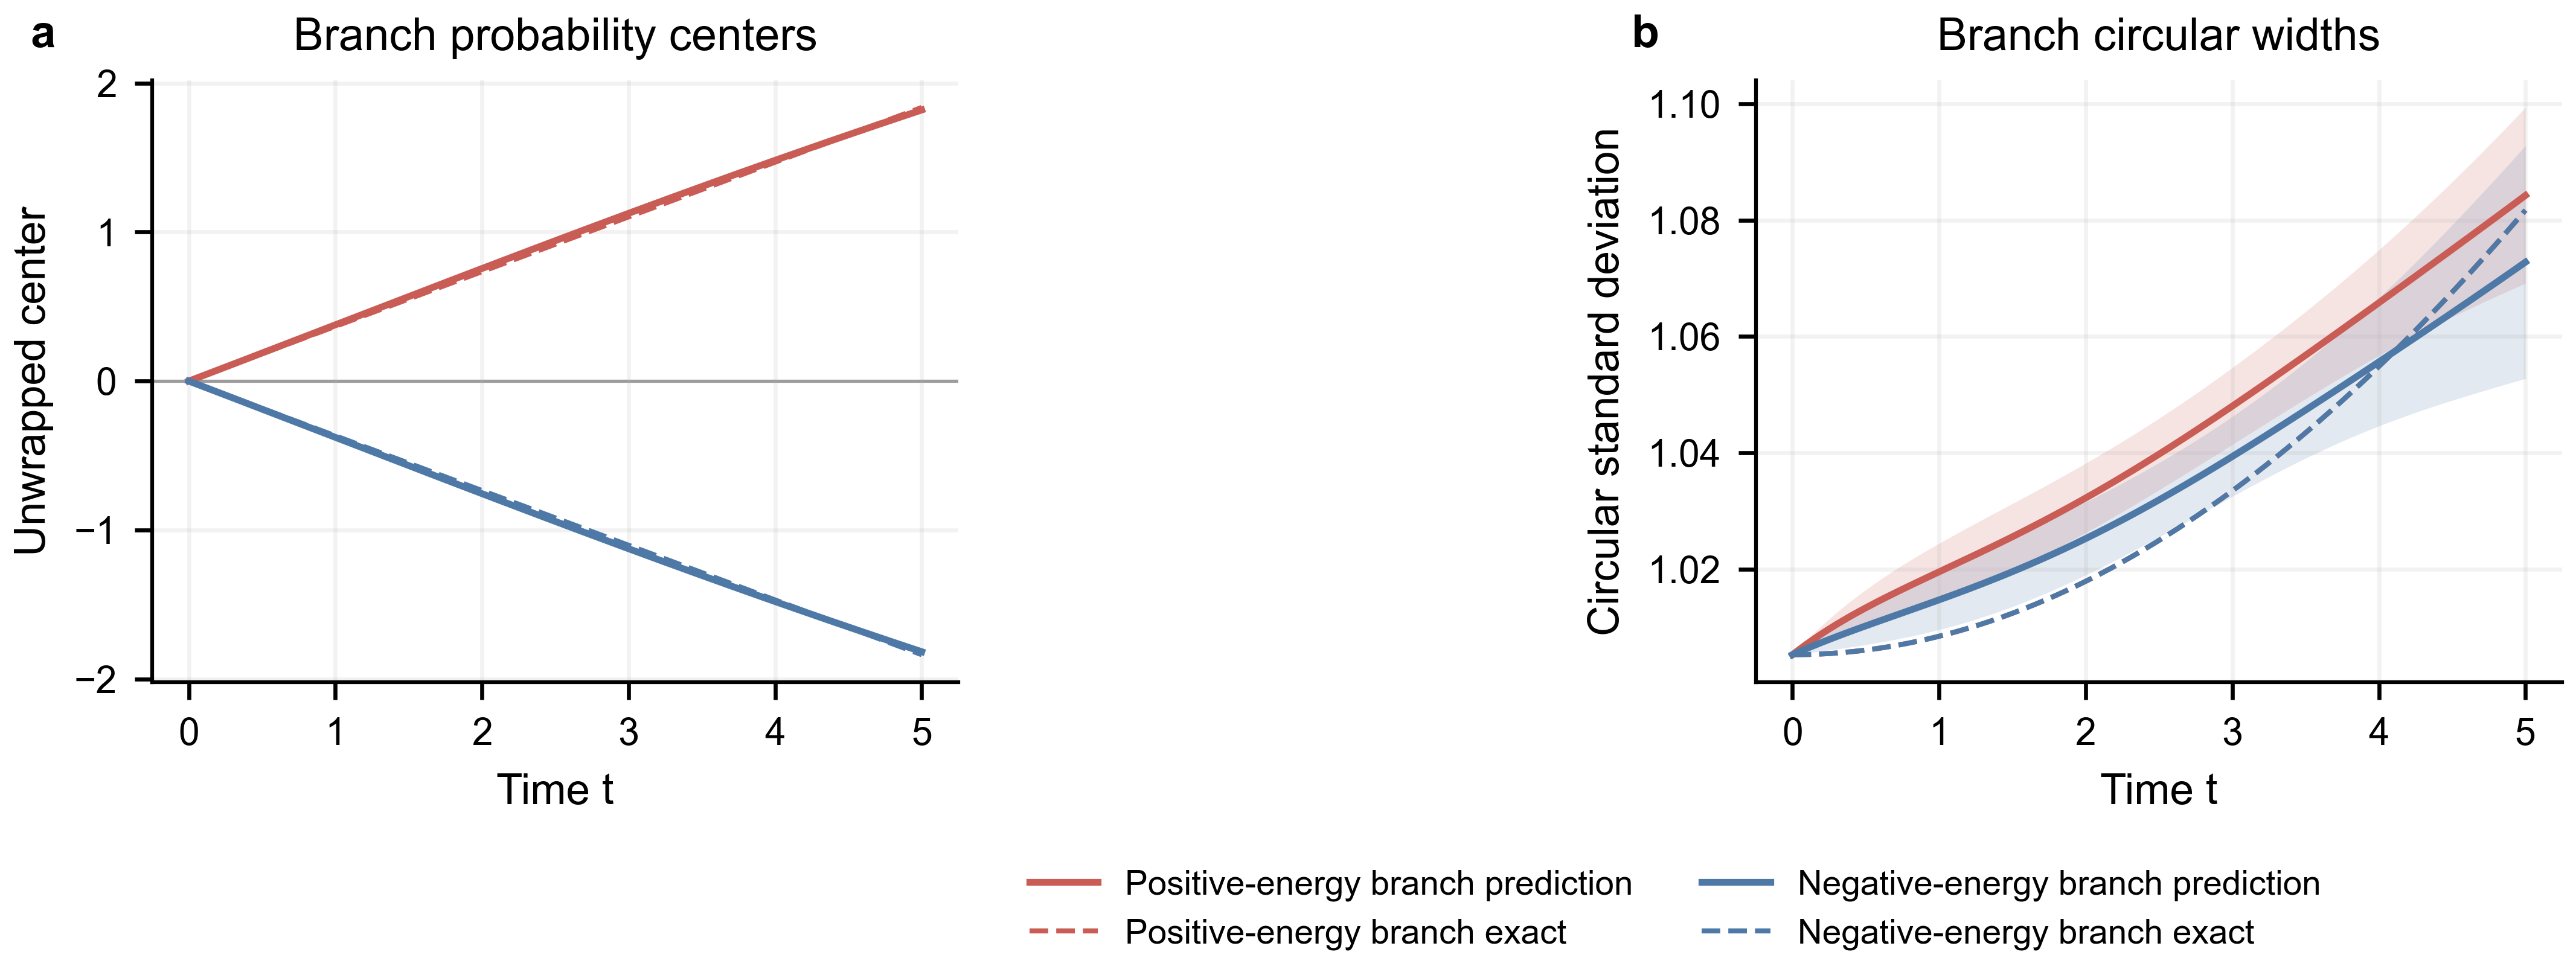
\includegraphics[width=0.88\textwidth]{results/figures/wavepacket_shared_spectral_ltpb/branch_center_width.png}
\caption{正、负能波包分别向相反方向传播，中心速度和宽度变化均通过预注册判据。}
\label{fig:wavepacket-branch}
\end{figure}

共享谱 LTPB 给出的正、负能波包平均群速度分别为 $+0.3665$ 和 $-0.3659$；未训练波数中点处的方程残差均方根为 $0.0017$--$0.0033$。旋量波函数误差由双波数实验中的 $0.0066$ 增至 $0.0410$，表明连续谱宽度增加后逼近难度上升。5 个随机种子所得波函数与概率流密度误差均较最佳对照模型低 10 倍以上。

\noindent\textbf{阶段结论：}
第六阶段满足全部预注册判据。相位表示已由离散能谱分量扩展到给定自由 Dirac 谱区间内的连续函数 $S_\pm(k,t)$；外势引起的动量通道耦合尚未纳入当前模型。

\section{阶段性结论}

\subsection{已获得的主要结论}

\begin{enumerate}
  \item \textbf{单一共同相位的适用范围：}该表示能够处理纯正能谱态；对于正、负能谱支叠加态，符号相反的快速时间相位仍有一部分保留在复振幅中，固定预算下的逼近误差因而增大。
  \item \textbf{能谱支分解的作用：}按自由 Dirac 哈密顿量的本征子空间分解旋量，并为各谱支设置独立相位函数，可准确恢复支间相对相位和概率流振荡。
  \item \textbf{关键结构：}等参数消融表明，能谱支对齐和逐支相位表示均与低误差密切相关；任一结构缺失时，当前基准中的误差均上升至高值平台。
  \item \textbf{已验证的适用范围：}该方法已由单波数叠加态推广至双波数离散谱，并进一步推广至给定自由谱区间内的高斯波包。
\end{enumerate}

\subsection{精度随问题复杂度变化}

\begin{table}[htbp]
\centering
\small
\caption{不同复杂度问题中的精度变化}
\begin{tabularx}{\textwidth}{@{}Y Y r r r@{}}
\toprule
问题 & 方法 & 旋量波函数误差 & 概率流密度误差 & 保真度 \\
\midrule
单波数正、负能谱支叠加 & LTPB & 0.0025 & 0.0046 & 0.999996 \\
双波数四能谱分量 & Multi-LTPB & 0.0066 & 0.0110 & 0.999965 \\
33 模态高斯波包 & Shared-Spectral-LTPB & 0.0410 & 0.0481 & 0.998249 \\
\bottomrule
\end{tabularx}
\end{table}

随着谱分量数目的增加，旋量波函数误差由 $0.0025$ 增至 $0.0410$，而保真度仍保持在 $0.998$ 以上。该趋势表明，逐支相位表示在当前自由问题中具有稳定作用，同时其精度余量随谱宽增加而减小。后续研究的核心问题是动量通道发生动态耦合时的相位表示与数值稳定性。

\subsection{与已有工作的关系及可能优势}

Kumar 等提出的 CPA-PINN 以 WKB 型相位--振幅分解处理半经典 Schrödinger 型方程，并利用连续性、质量和能量守恒约束提高波函数重构与含噪参数反演的稳定性\cite{kumar2026}。对于标量 Schrödinger 波函数，概率流显含共同相位的空间梯度。Dirac 概率流密度由旋量双线性型 $\psi^\dagger\sigma_x\psi$ 给出，整体相位在该双线性型中约去。本方法保留快速相位与缓变振幅分离的思想，并以 Dirac 哈密顿量的正、负能谱投影作为相位分解的物理依据。由此推测，其主要优势将出现在含有多能谱支相干的长时间演化问题中。

Lorin 和 Yang 已建立较一般的含时 Dirac-PINN 框架，直接以神经网络逼近旋量波函数，并讨论范数约束、弯曲时空和费米子倍增等问题\cite{lorin2022}。该表示对解的谱结构要求较少。LTPB 在已知自由能谱结构时引入更强的物理先验，将快速时间相位从缓变系数中分离。当前等预算实验中，单模混合态的旋量波函数误差由 SP-CPA 的 $0.7991$ 降至 $0.0025$，33 模态波包的误差较最佳可训练对照模型低约 22 倍。这些结果支持以下推断：对于谱结构可辨认的强振荡 Dirac 问题，能谱支坐标可能改善优化条件和长时间相位精度。

傅里叶伪谱、多尺度时间积分等传统方法在自由演化和非相对论极限中已形成具有严格误差估计的高精度正向求解框架\cite{bao2016}。当前实验尚未给出 LTPB 在单次正向求解成本上的优势。其潜在用途主要包括将方程约束与稀疏、含噪观测统一纳入训练过程，构造可连续求导的时空代理模型，以及在同一框架内实施状态重构和参数反演。上述用途属于待检验的研究假设。

\section{下一阶段计划}

\subsection{阶段七：弱且光滑的周期外势}

首先考虑周期标量势
\begin{equation}
V(x)=V_0\cos(qx)I_2.
\end{equation}
谱空间中相邻动量通道满足
\begin{equation}
i\partial_t\widetilde\psi_k=
H(k)\widetilde\psi_k+\frac{V_0}{2}
\left(\widetilde\psi_{k-q}+\widetilde\psi_{k+q}\right).
\end{equation}
该模型在保持外势光滑和物理机制清楚的条件下，引入了非平凡的动量转移。实验将考察共享谱 LTPB 对模态占据数交换、概率流密度及谱支相干项的恢复能力。低占据或新生模态附近的振幅趋近于零，极坐标相位可能出现病态；相应的改进方向包括零振幅邻域的相位正则化以及复数表示与极坐标表示的混合参数化。

\subsection{后续阶段}

\begin{itemize}
  \item \textbf{阶段八：}加入稀疏、含噪的概率密度或概率流观测，研究状态重构以及质量参数 $m$、外势参数的反演。
  \item \textbf{阶段九：}与自适应采样 PINN、损失平衡方法、傅里叶谱方法和分裂算子法进行统一基准评测。
  \item \textbf{阶段十：}系统整理理论依据、算法结构、消融实验、适用范围、数据实验、计算复杂度和适用性边界，形成投稿材料。
\end{itemize}

\section{当前结论的适用范围}

现有实验支持如下结论：在一维自由 Dirac 方程、给定傅里叶表示及固定训练预算下，能谱支对齐的独立可学习相位可显著降低正、负能谱支叠加态的旋量波函数、概率流密度及相对相位误差。

尚待验证的内容包括：
\begin{itemize}
  \item 从数据和方程残差中自动辨识未知能谱及本征子空间；
  \item 一般外势、高维及强耦合 Dirac 方程中的有效性；
  \item 相对于成熟谱方法或分裂算子法的正向求解精度与计算效率；
  \item 方法的普适性、严格首创性及可复现实验边界。
\end{itemize}

若以 SCI 二区至三区或同等级会议为投稿目标，仍需完成外势耦合主实验、稀疏含噪数据应用、传统求解器对照及完整的计算成本分析。

\enlargethispage{4\baselineskip}
\begin{thebibliography}{9}
\raggedright
\footnotesize

\bibitem{kumar2026}
S. Kumar, H. K. Dwivedi, and Rajeev,
\emph{Structure-preserving conservative phase-amplitude PINNs for semiclassical Schrödinger-type equations},
\textit{Journal of Computational and Applied Mathematics}, vol. 485, 117607, 2026.
\href{https://doi.org/10.1016/j.cam.2026.117607}{doi:10.1016/j.cam.2026.117607}.

\bibitem{lorin2022}
E. Lorin and X. Yang,
\emph{Time-dependent Dirac equation with physics-informed neural networks: Computation and properties},
\textit{Computer Physics Communications}, vol. 280, 108474, 2022.
\href{https://doi.org/10.1016/j.cpc.2022.108474}{doi:10.1016/j.cpc.2022.108474}.

\bibitem{bao2016}
W. Bao, Y. Cai, X. Jia, and Q. Tang,
\emph{A uniformly accurate multiscale time integrator pseudospectral method for the Dirac equation in the nonrelativistic limit regime},
\textit{SIAM Journal on Numerical Analysis}, vol. 54, no. 3, pp. 1785--1812, 2016.
\href{https://doi.org/10.1137/15M1032375}{doi:10.1137/15M1032375}.

\end{thebibliography}

\section{原始材料}

\begin{itemize}
  \item 开题报告：CPA-PINN 推广至 Dirac 方程的局限与旋量双相位方法。
  \item CPA 直接迁移实验报告：\path{EXPERIMENT_REPORT.md}
  \item LTPB 初步实验报告：\path{LEARNED_TWO_PHASE_PILOT_REPORT.md}
  \item 机制消融预注册：\path{LTPB_MECHANISM_ABLATION_PREREGISTRATION.md}
  \item 机制消融实验报告：\path{LTPB_MECHANISM_ABLATION_REPORT.md}
  \item 双波数实验预注册：\path{MULTIMODE_LTPB_PREREGISTRATION.md}
  \item 双波数实验报告：\path{MULTIMODE_LTPB_EXPERIMENT_REPORT.md}
  \item 连续波包实验预注册：\newline
  \path{WAVEPACKET_SHARED_SPECTRAL_LTPB_PREREGISTRATION.md}
  \item 连续波包实验报告：\newline
  \path{WAVEPACKET_SHARED_SPECTRAL_LTPB_REPORT.md}
\end{itemize}

本文使用的图片均直接引用项目现有 \texttt{results/figures/} 目录。

\end{document}
